\documentclass[11pt,a4paper]{article}
\usepackage[margin=3cm]{geometry}
\usepackage[english]{babel}
\usepackage[dvipsnames]{xcolor}
\usepackage[utf8x]{inputenc}
\usepackage{amsmath}
\usepackage{graphicx}
\setlength {\marginparwidth }{2cm}
\usepackage[colorinlistoftodos]{todonotes}
\usepackage{setspace}
\usepackage{etoolbox}
\usepackage{framed,color}
\usepackage{tcolorbox}
\usepackage[english]{babel}
\usepackage[nottoc]{tocbibind}
\usepackage{float}
\usepackage{pdfpages}
\renewcommand{\baselinestretch}{1.3}

\begin{document}

\begin{titlepage}

\newcommand{\HRule}{\rule{\linewidth}{0.5mm}} % Defines a new command for the horizontal lines, change thickness here

\center % Center everything on the page

%----------------------------------------------------------------------------------------
%	HEADING SECTIONS
%----------------------------------------------------------------------------------------

\textsc{\LARGE New Zealand}\\[0.5cm]

\textsc{\LARGE  Maritime School}\\[1.5cm]
\textsc{\Large ETO Course 942.467}\\[0.2cm] % Major heading such as course name
\textsc{\large Electrical Maintenance and Repair Procedures}\\[0.5cm] % Minor heading such as course title

%----------------------------------------------------------------------------------------light
%	TITLE SECTION
%----------------------------------------------------------------------------------------

\HRule \\[0.5cm]
{ \huge \bfseries Module Assignment}\\[0.2cm] % Title of your document
\HRule \\[0.5cm]
\begin{minipage}{0.4\textwidth}
\begin{flushleft} \large
\emph{Author:}\\
Levi \textsc{Dubbelman}

\textit{SN: 190000929}\par
\textit{Special thanks to:}\par
Toby \textsc{Swann-McKay}\par
\& Lewis \textsc{Gould}
\end{flushleft}
\end{minipage}
~
\begin{minipage}{0.4\textwidth}
\begin{flushright} \large
\emph{Supervisors:} \\
John \textsc{Lamb} \&

Nick \textsc{Cossar}
\end{flushright}
\end{minipage}\\[2cm]
{\large April, 2019}\\[2cm]

\includegraphics[width=4cm]{logo.png}
\vfill

\end{titlepage}

\tableofcontents
\newpage

\section*{Introduction}light
\begin{tcolorbox}[colback=red!5!white,colframe=red!75!black,title=\textbf{Brief}]
Research each of the Four Learning Outcomes and answer with your interpretation.
Use reading material provided on Canvas, library material or other suitable sources. Where possible provide reference to the sources. Email back to the tutor when complete.
\end{tcolorbox}
\begin{abstract}
\textbf{Background}

This module addresses the correct safe operating procedures technical staff should undertake before commencing work on any electrical equipment, as well as the hazards that may exist whilst working on electrical equipment. Special attention is also paid to fire control systems, and the technical drawings and schematics, as well as how to apply them effectively when performing work.

\textbf{Scope}

This assignment contains an overview of accepted and safe practices that may be applied to any electrical equipment, the various equipment (P.P.E.) and accessories associated with maintenance and repairs.

\textbf{Aim}

This document's aim is to provide a simplified overview of the approach one should take when dealing with electrical equipment, the various categories or levels of protection one might require, and a general informative guide for maintenance and repairs.
\end{abstract}
\newpage
% BEGINNING OF LEARNING OUTCOME 1
\section{Learning Outcome 1}
\begin{tcolorbox}[colback=red!5!white,colframe=red!75!black,title=\textbf{Demonstrate knowledge of safety precautions to take prior to undertaking shipboard electrical maintenance and repair work}]
\begin{itemize}
\item Identify safety hazards which can be present when working on shipboard electrical equipment.
\item Name proper Personal Protective Equipment (PPE) to be used when working on various shipboard electrical equipment.
\item Explain Lockout-Tagout procedures prior to electrical maintenance and repair work.
\item Explain use of fixed and portable earthing devices and how to apply them safely.
\item Explain safe electrical maintenance/repair work procedures for flammable areas.
\item Explain how to interpret and follow shipboard instructions relating to electrical maintenance and repair work.
\item Explain how to interpret and follow electrical equipment/manufacturer safety guidelines for repair and maintenance work.
\end{itemize}
\end{tcolorbox}
\subsection{Hazards}
\subsubsection{Electric Shock}
Of all hazards present when working on, or near, electrical equipment, shock hazards can be the most severe threat to technical staff. When passing through a human body, Currents of approximately 0.2 A are potentially fatal, because they can make the heart fibrillate, or beat in an uncontrolled manner. Other injuries may occur at other points in the body if bypassing the heart. These generally require greater currents. However, resistance in human bodies is inversely proportional to current applied -- that is, the longer and more intense the electromotive force, the lower the human body's resistance to the current will be.\cite{cutnell} In general, for limb-contact electrical shocks, accepted rules of thumb are: 1-5 mA is the level of perception; 10 mA is the level where pain is sensed; at 100 mA severe muscular contraction occurs, and at 100-300 mA electrocution occurs.\cite{carr}
\subsubsection{Arc Blast}
An arc blast (sometimes referred to as arc flash, or flash-over) is an umbrella term for the release of both light and heat energy resulting from an arc fault. A detonation or discharge occurs as a result of a low impedance connection to ground or a different phase across the aether. One of the most common causes of arc-flash injuries occurs when switching on electrical circuits, especially tripped circuit breakers. To avoid this, the fault must be isolated before energizing the circuit. An arc blast may also occur in energized circuits whilst testing and occur due to conductive debris being present. Arc blasts generally do not occur at voltages lower than 220 V, but their likelihood increases exponentially in proportion to the electromotive force in the circuit, as does the distance over the aether the arc fault may occur. The best defense against an arc blast is proper and thorough isolation of any circuit with which an arc fault occurs. Failing this, P.P.E. may be a technician’s last line of defense. Arc Blast body suits are available and should be worn when working on any circuit of sufficiently high voltage (440V or greater) where there is risk of an arc blast.

\subsubsection{Transient Over-voltage}
“Over-voltage” is the term used to describe voltage in a circuit which exceeds the maximum voltage, or upper design limit for the particular circuit. Transient over-voltage is a short burst of energy which may occur naturally, especially from lightning, or man-made. These man-made spikes of over-voltage generally occur when inductive loads, such as electric motors or electromagnets. Transient over-voltages significantly degrade and damage electronic systems, and may result in a fire, or electric shock from a flash-over if insulation is worn down sufficiently. While generally most ships will have Surge Protection Devices (SPDs), these may need to be replaced if they suffer a great enough over-voltage. In addition, as the majority of motors on board ships are Direct On Line (D.O.L.) starters, over-voltage concerns are a regular occurrence.
\begin{center}
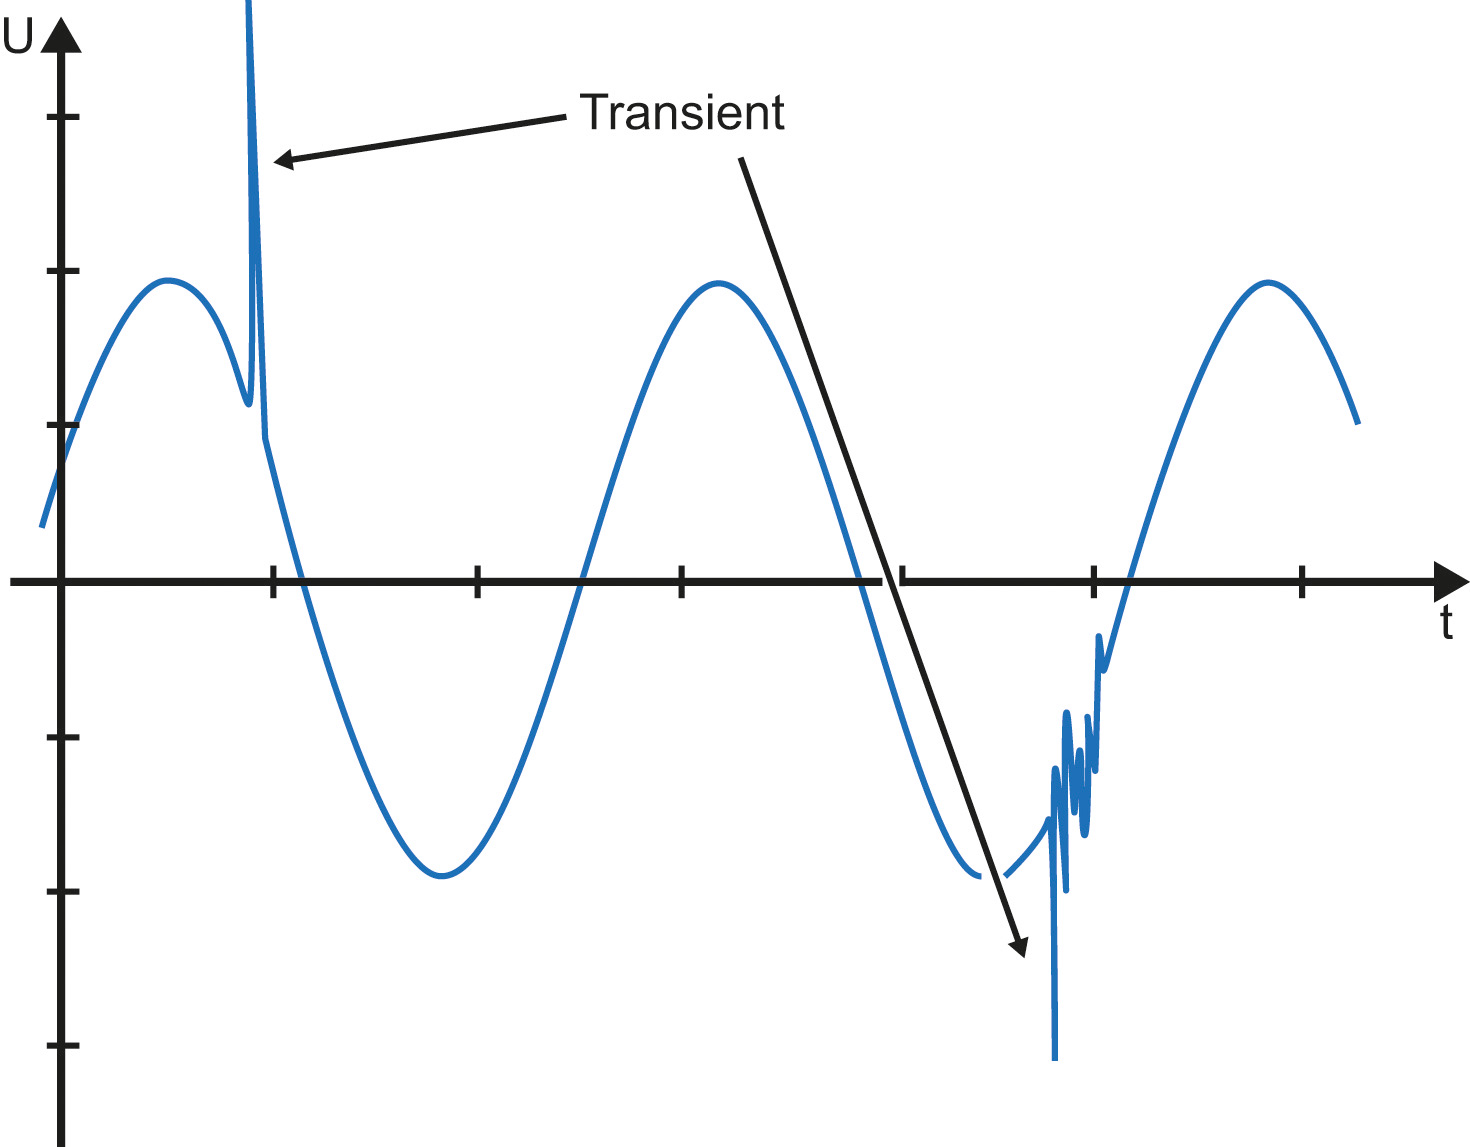
\includegraphics[width=8cm]{transient}
\end{center}
\subsubsection{Electrolysis}
Electrolysis is the process by which a chemical change is induced in a material by way of passing an electric current through it. Sometimes, this process of displacing electrons is known as oxidation. When an electron is displaced, it renders the material inert of charge, also known as neutral. At sea, we are able to combat electrolysis with sacrificial anodes. Seawater acts as an electrolyte and displaces electrons from the sacrificial anode, oxidizing and producing a protective layer. We apply this method to the ship’s hull, the ballast tanks, heat exchangers, etc. Nearly any metal which is likely to encounter a significant amount of corrosion via electrolysis. We often use zinc as the primary metal in the sacrificial anode. Identifying and reporting corrosion to your immediate superior is incredibly important, and will prevent further damage from occurring.
\begin{center}
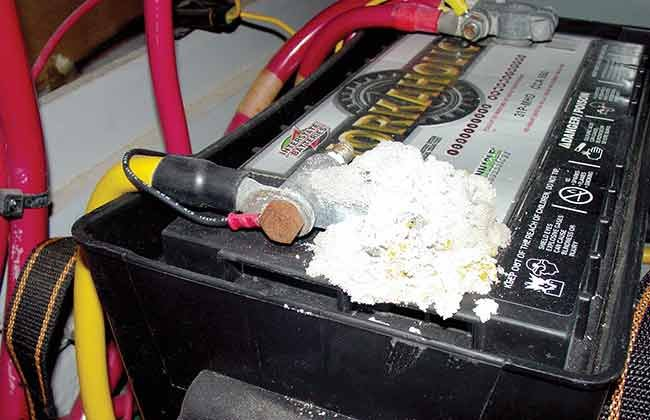
\includegraphics[width=8cm]{electrolysis}\par
A corroded battery.
\end{center}
\subsection{Weather}
\subsubsection{Rain, Seawater, and Humidity}
Rain, seawater and humidity are able to cause corrosion, and weaken the structural integrity of the ship, or cause systems to fail. They can also create hazards with which we must be aware of and prepare for. Heavy rains may cause visibility issues, making the important of correctly functioning lighting absolutely paramount. It will also cause surfaces to become slippery, and dangerous to tread on. Ensuring that you use the hand-railing provided is extremely important, as well. Rain may also cause moisture buildup inside sensitive electronics. In the case of induction motors, ensuring their heaters are functioning correctly and regularly maintained is also very important. In the case of lighting, water may pool at the bottom of the light fixture’s enclosure. In this instance, regular maintenance and checking of seals will help. Additional moisture present on our bodies will also lower our internal resistance against electric current, which may greatly increase the amount of current which can pass through our bodies if we were to be electrocuted.
\subsubsection{Temperature}
As with the weather, temperatures may vary greatly at sea. It is important to understand the limitations of the electronics and machinery aboard ships. Many components have thermal protection units (TPUs) whose maximum safe operation temperatures may be within the realm of achievable in specific times and places throughout your voyage. It is important to understand that the temperature of a machine will always combine with the ambient temperature. For example, an engine who, at 0 degrees centigrade, has a thermal protection unit which trips at 100 degrees centigrade, and produces enough heat to operate between 50-70 degrees centigrade may actually reach a high enough temperature to trip the TPU on a hot 30-40 degrees centigrade day. It is important to treat every alarm with the severity of a fire until you are able to disprove it is not. On the other hand, during extremely cold seasons, systems may not be able to work at all. In this instance, keeping system heaters well maintained and working when the unit is not in use is absolutely critical to ensuring smooth operations and machine longevity. Temperature may also cause fatigue, heat stroke, or heat syncope in workers. Ensuring that regular breaks are taken, and all workers are sufficiently hydrated may save lives.
\subsection{Other Hazards}
\subsubsection{Corrosion}
A Sodium Chloride (salt, $NaCl$) and hydrogen hydroxide (water, $H_2O$) solution is electrically conductive. Salt ions are able to transport electrical charge, allowing galvanic corrosion to occur rapidly, and short circuiting to occur when live circuitry is submerged in it. At sea, it is inevitable that corrosion will occur. We have methods to reduce this corrosion, like sacrificial anodes, but it is a technician's duty to keep a rigorous schedule of preventative maintenance throughout the ship. Ensuring all seals do not allow the passage of water, as well as stopping any circuits exposed to salt water from being energized.
\subsubsection{Movement of Ship}
When working on a ship, it is important to understand the dynamics of being aboard a vessel capable of sudden, immediate movement on any axis. Rolling (rotational movement across the $X$ axis) and pitching (rotational movement across the $Z$ axis) may occur unexpectedly. It is important for technicians to ensure the appropriate level of P.P.E. for the job they are doing. In a situation where sudden movement causes the technician to lose balance, he may, consequently, fall into or onto live circuitry, or strike an object with considerable force. When working in compromising positions, e.g. atop a crane, that a harness is fitted at all times. Furthermore, understanding the degradation of electronics by repetitive kinetic motion is critical to quickly and effectively locating and repairing ground faults on the vessel. In addition, proper stowing of equipment and tools when work is completed is critical in ensuring that they are not misplaced or potentially create a hazard when left unattended.
\subsubsection{Pipe Leakage}
Depending on the fluid expelled, a pipe leakage may pose a hazard in a plethora of different ways. Waste-water pipes pose a bio-hazard and disease risk. Fuel pipes may be a bio-hazard and fire risk, and also have the potential to dissolve or greatly weaken insulation on any wires it may come in contact with, as well as potentially exposing aquatic life to harmful pollution. Steam pipes are a thermal risk and may endanger anyone near the pipe. If the temperature and pressure are great enough, steam pipes may also act as a powerful kinetic force, able to cut or seriously maim anyone it strikes. It is essential that the technician understand the location and operation of fire control units, as well as the control pumps for all pipes. Prior knowledge and understanding is your best defense against pipe leakages, as swift disabling of any existing flow is the most important step in damage control.
\subsubsection{Gases \& Fumes}
Depending on the type of ship, it may be carrying hazardous cargo, such as on chemical or oil tankers. It is therefore critical to ensure that a breathing apparatus is affixed when working near these tanks. Short-term problems include dizziness, shortness of breath, unconsciousness, and, in severe cases, death. Long-term problems may include increased exposure to known carcinogens, respiratory irritation (nosebleeds, ulcers, and holes in the nasal septum in extreme cases), blood poisoning, metal fume fever, kidney and bone defects, nervous system disorders, and pulmonary edema (fluid in the lungs). In poorly ventilated areas, gases and fumes also displace oxygen. These may also be a skin irritant, and additional P.P.E. may be required.
\subsubsection{Potentially Hazardous Energy}
If the potential exists for the release of hazardous stored energy or for the re-accumulation of stored energy to a hazardous level, the technician must take steps to prevent injury from the release of said energy. Energy in any form becomes hazardous when it builds to a dangerous level or is released in any quantity that could injure a worker. Workers servicing or maintaining machines or equipment may be seriously injured or killed if hazardous energy is not properly controlled. Injuries resulting from the failure to control hazardous energy during maintenance activities can be serious or fatal. Injuries may include electrocution, burns, crushing, cutting, lacerating, amputating, or fracturing body parts, and others.

It's important to understand that electricity is not the only form of hazardous energy employees may encounter. Main energy sources that supply power to the entire machine or equipment may be electrical, but secondary energy sources such as pneumatic or mechanical energy may still be stored with the potential to cause injury.

\begin{itemize}
    \item \textbf{Electrical}

    Exposed, or live circuitry or wires. Equipment not fully de-energized. Electrostatic charge.
    \begin{center}
    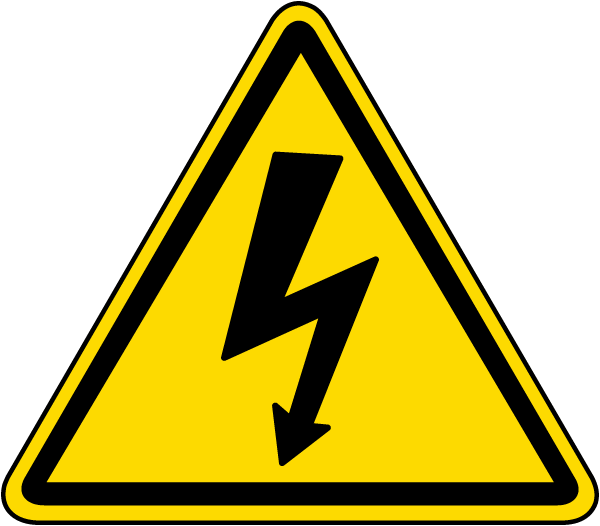
\includegraphics[width=3cm]{shock}
    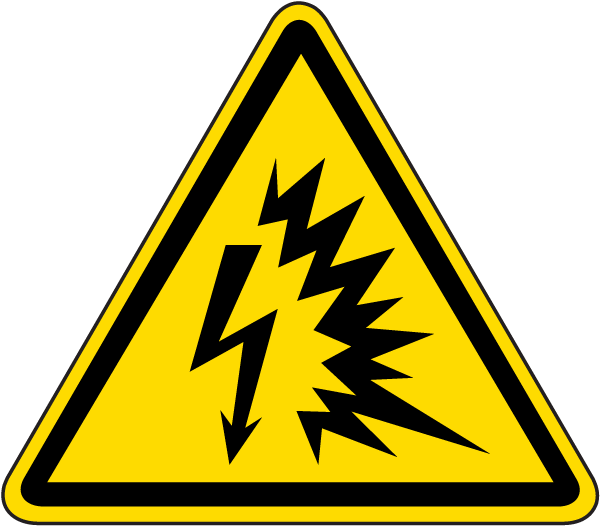
\includegraphics[width=3cm]{shock2}
    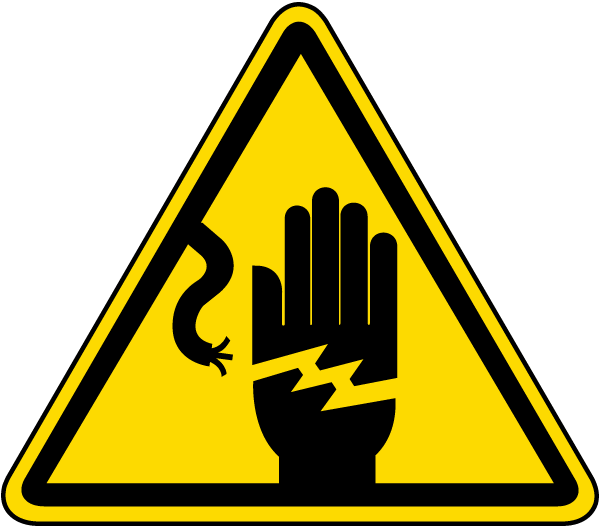
\includegraphics[width=3cm]{shock3}
    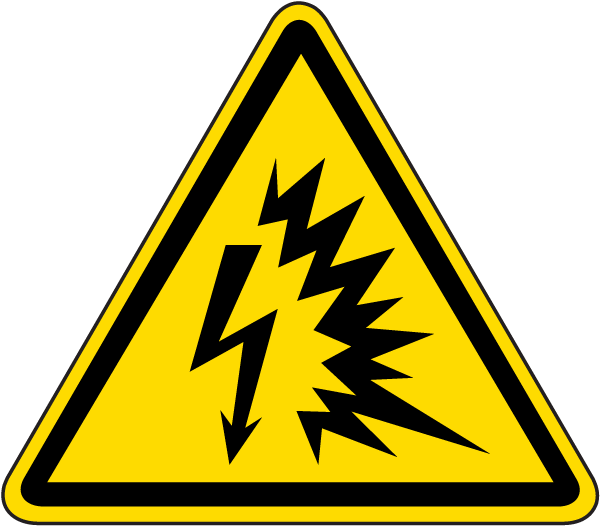
\includegraphics[width=3cm]{shock4}
\end{center}
    \item \textbf{Chemical}

    Liquids, such as diesel, acids, and caustics. Gases, such as natural gas. Solids, such as wet and dry cell batteries, and combustible dust.
    \begin{center}
    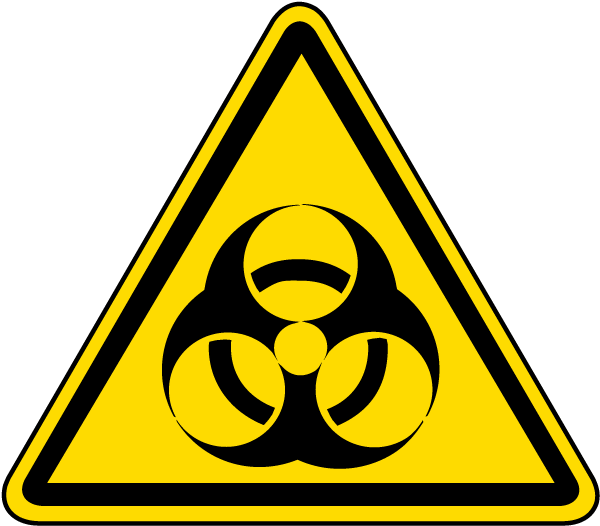
\includegraphics[width=3cm]{chemical}
    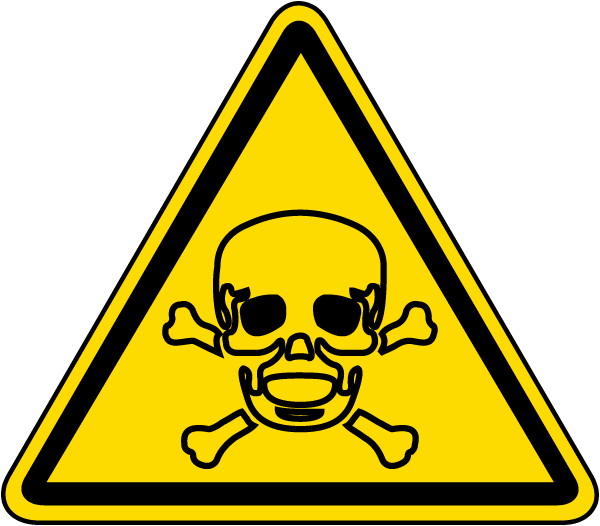
\includegraphics[width=3cm]{chemical2}
        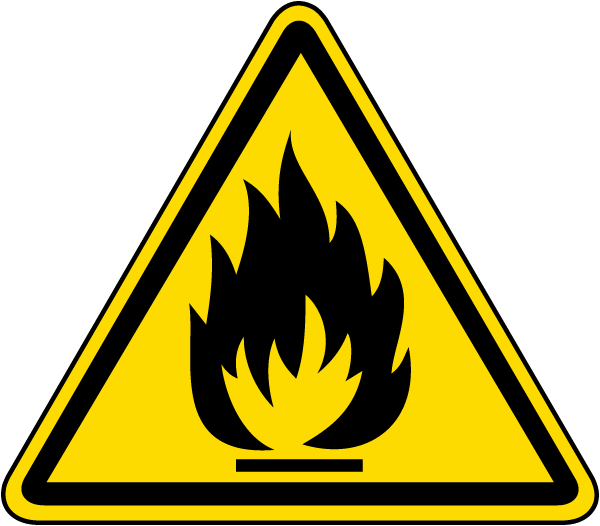
\includegraphics[width=3cm]{flammable}
\end{center}
    \item \textbf{Gravitational}

    Objects supported by a crane, and elevated platforms. Potential energy is converted to kinetic energy.
    \begin{center}
    
\includegraphics[width=3cm]{gravity}
\end{center}
    \item \textbf{Hydraulic}

    Pressurized hydraulic systems, including hoses, pumps, valves, and actuators.
    \begin{center}
    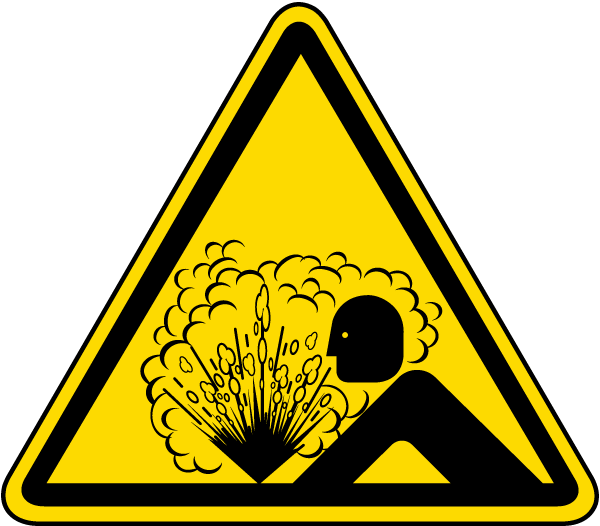
\includegraphics[width=3cm]{hydraulic}
        
\includegraphics[width=3cm]{hydraulic2}
\end{center}
    \item \textbf{Mechanical}

    Sources such as a spring under compression. Extreme sound is also a hazardous mechanical energy.
    \begin{center}
    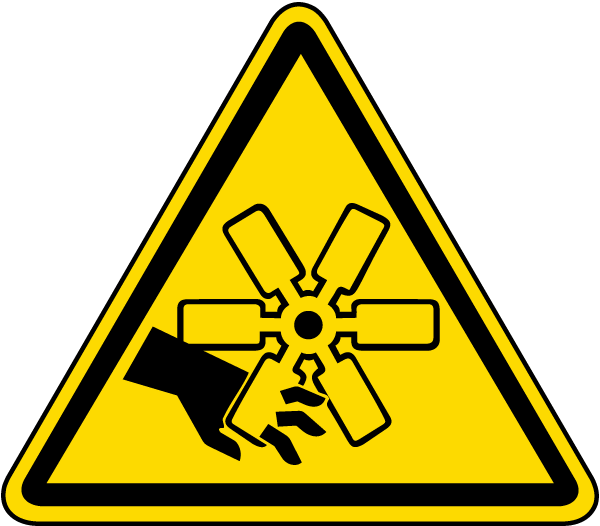
\includegraphics[width=3cm]{rotating1}
    
\includegraphics[width=3cm]{rotating2}
        
\includegraphics[width=3cm]{rotating3}
\end{center}
    \item \textbf{Pneumatic}

    Pressurized air or gas systems, including pipes, pumps, valves, actuators, and air compressors, and tank and pipe purging systems.
    \begin{center}
    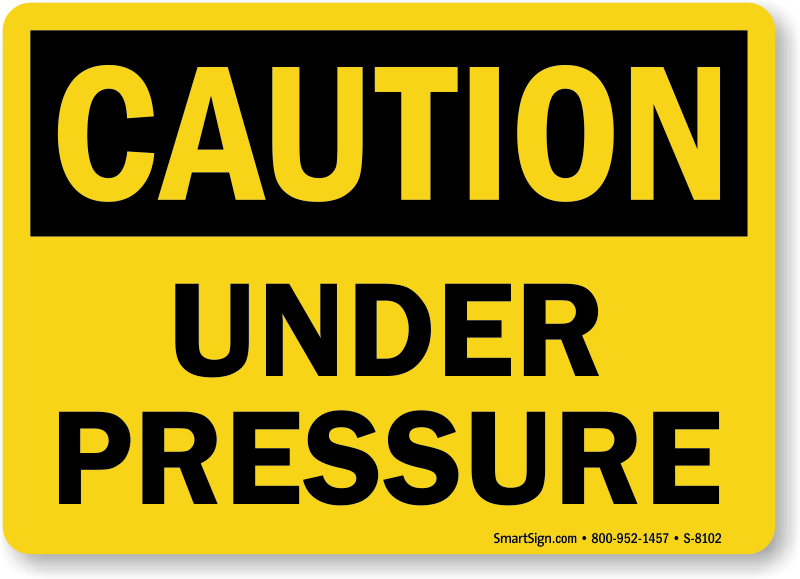
\includegraphics[width=3cm]{pressure.png}
        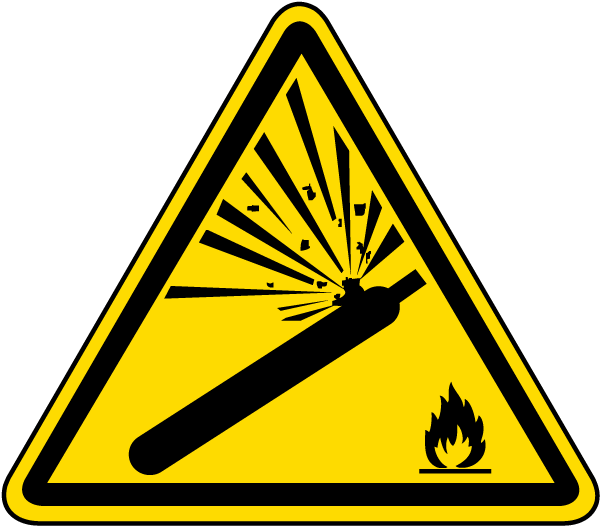
\includegraphics[width=3cm]{pneumatic}
            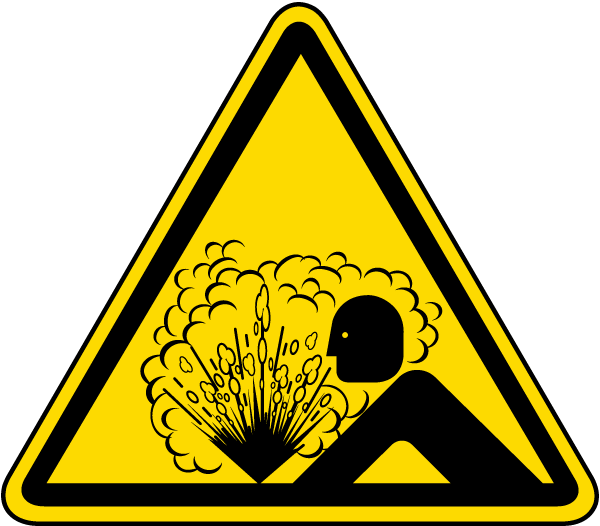
\includegraphics[width=3cm]{hydraulic}
\end{center}
    \item \textbf{Radiant}

    Energy that travels by waves or particles, particularly electromagnetic radiation such as heat or x-rays. Ionizing radiation includes alpha and beta particles, computed tomography (CT) and X-rays.
    \begin{center}
    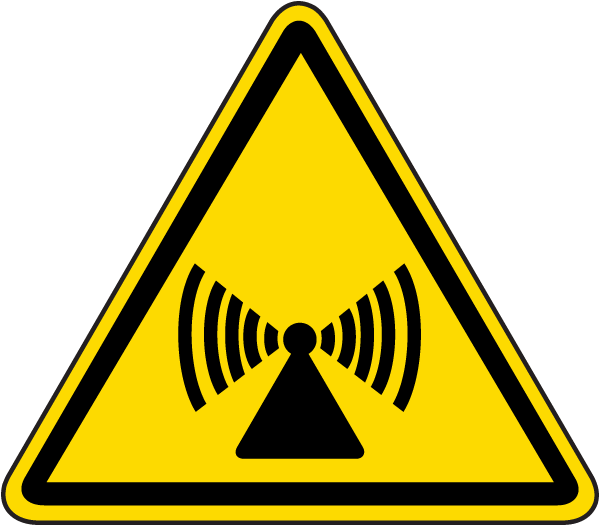
\includegraphics[width=3cm]{radiant}
    
\includegraphics[width=3cm]{radiant2}
    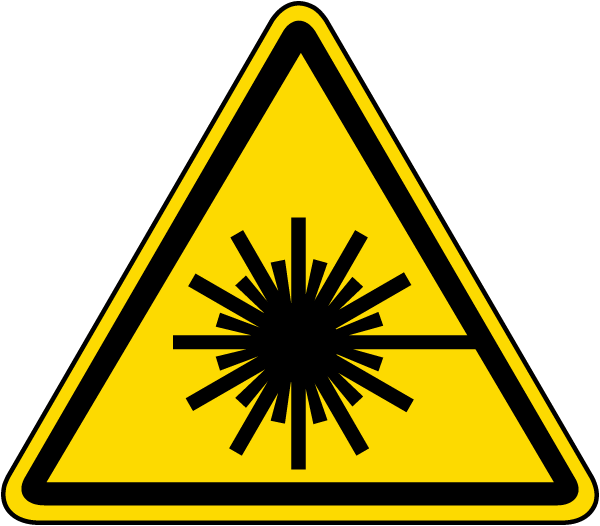
\includegraphics[width=3cm]{radiant3}
    
\includegraphics[width=3cm]{radiant4}
\end{center}
    \item \textbf{Thermal}

    Hot water, heated oil, steam, and equipment need time to cool, while liquefied gases, such as nitrogen, need time to warm to safe thermal levels.
    \begin{center}
    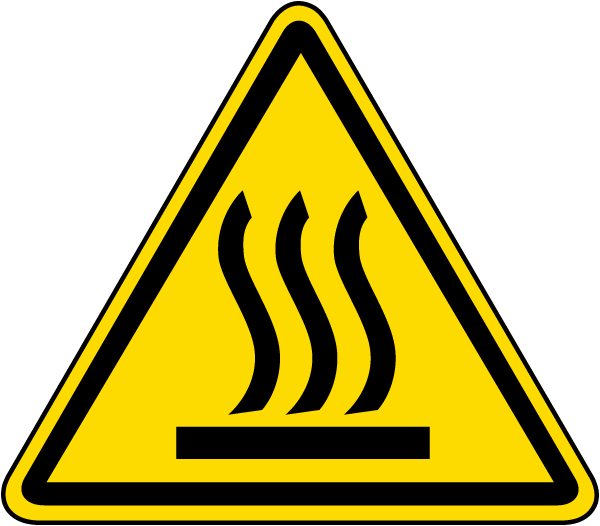
\includegraphics[width=3cm]{thermal}
    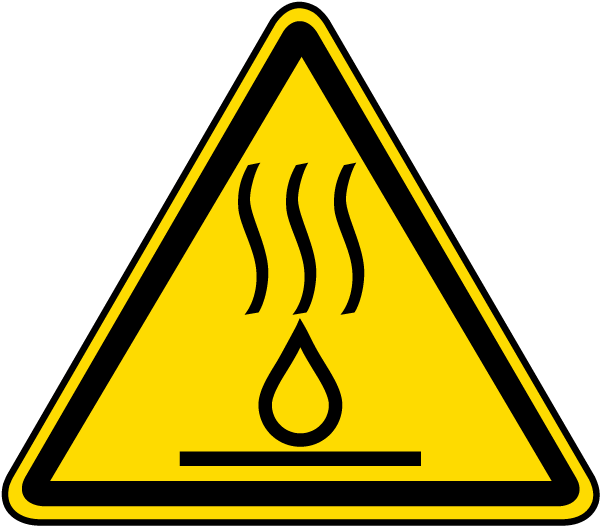
\includegraphics[width=3cm]{thermal2}
        
\includegraphics[width=3cm]{thermal3}
\end{center}
    \item \textbf{Explosive}

    The rapid increase in the volume of energy with the generation of high temperatures and the release of gases. Supersonic explosions are called detonations. Subsonic explosions are called deflagration. A boiling liquid vapor expanding explosion is called “B.L.E.V.E.”
    \begin{center}
    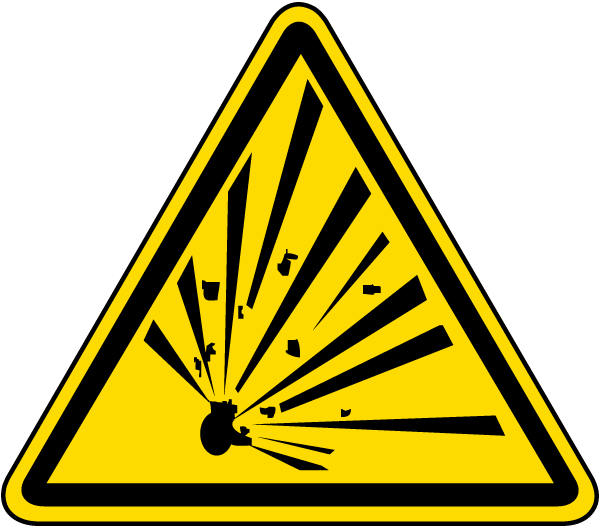
\includegraphics[width=3cm]{explosive}
\end{center}
\end{itemize}
\subsection{Personal Protection Equipment (P.P.E.)}
P.P.E. may be used for technical staff performing work on or near electrical equipment and varies with the level of voltage present. At extremely low voltages, such as 0-9V, it may even be preferable for technical staff to intentionally increase their effectiveness as a ground, or to eliminate electric potential, in order to prevent electrostatic damage to sensitive components, such as microprocessors, or prevent electrostatic discharge when working with extremely flammable chemicals. This can be achieved using ESD devices, such as footwear, wristbands or mats.
\begin{center}
  
\includegraphics[width=8cm]{esd.jpg}\par
An ESD Wristband.\par The crocodile clip connects to the same ground as the components the work is being performed on.
  \end{center}

On circuitry where electromotive forces greater than 0-24V exist, it may be required under your company's S.O.P., as well as being good safety practice, to equip greater levels of P.P.E.

These can be defined by "Hazard Risk Categories" and range from 1, the lowest risk, to 4, the highest risk.
\begin{center}
  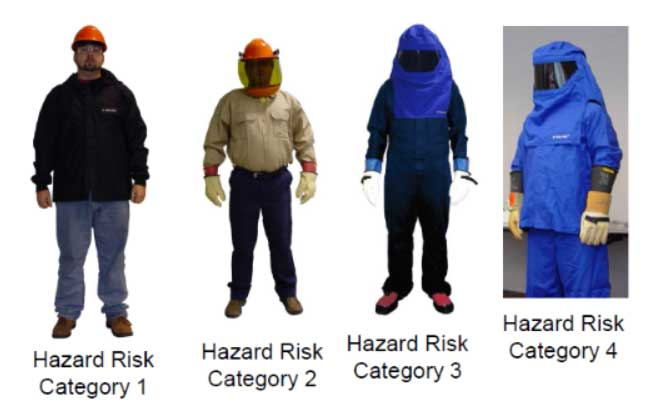
\includegraphics[width=12cm]{riskcat.jpg}\par
The Hazard Risk Categories for Electrical Safety.
  \end{center}

\subsubsection*{Eye Protection}
Eye protection is required whenever there is danger of injury to the eyes or face from arc flash or from flying objects resulting from electrical explosion. Safety glasses for electrical work should be non-conductive, anti-fogging, anti-scratch and anti-static with 99.9\% UV protection. Goggles are intended for eye protection only - they do not provide any face protection. If working where there is a threat of injury to the eyes and face from electrical arc flash, safety glasses and goggles should be used with an Arc Flash Hood, hard hat, and arc rated face shield with chin cup.
\begin{center}
  
\includegraphics[width=8cm]{glasses.jpg}\par
  \end{center}
\subsubsection*{Hard Hats}
OSHA standards mandate that a hard hat must be worn "when working in areas where there is a potential for injury to the head from falling objects." Hard hats must also be worn in working areas where there is the risk of exposure to electrical conductors that can potentially contact the head. Class E Hard Hats are designed to reduce exposure to high voltage conductors, and offer dielectric protection up to 20,000 volts (phase to ground). This amount of voltage protection is designated to the head only, and is not an indication of the overall voltage protection allocated to the worker.
\begin{center}
  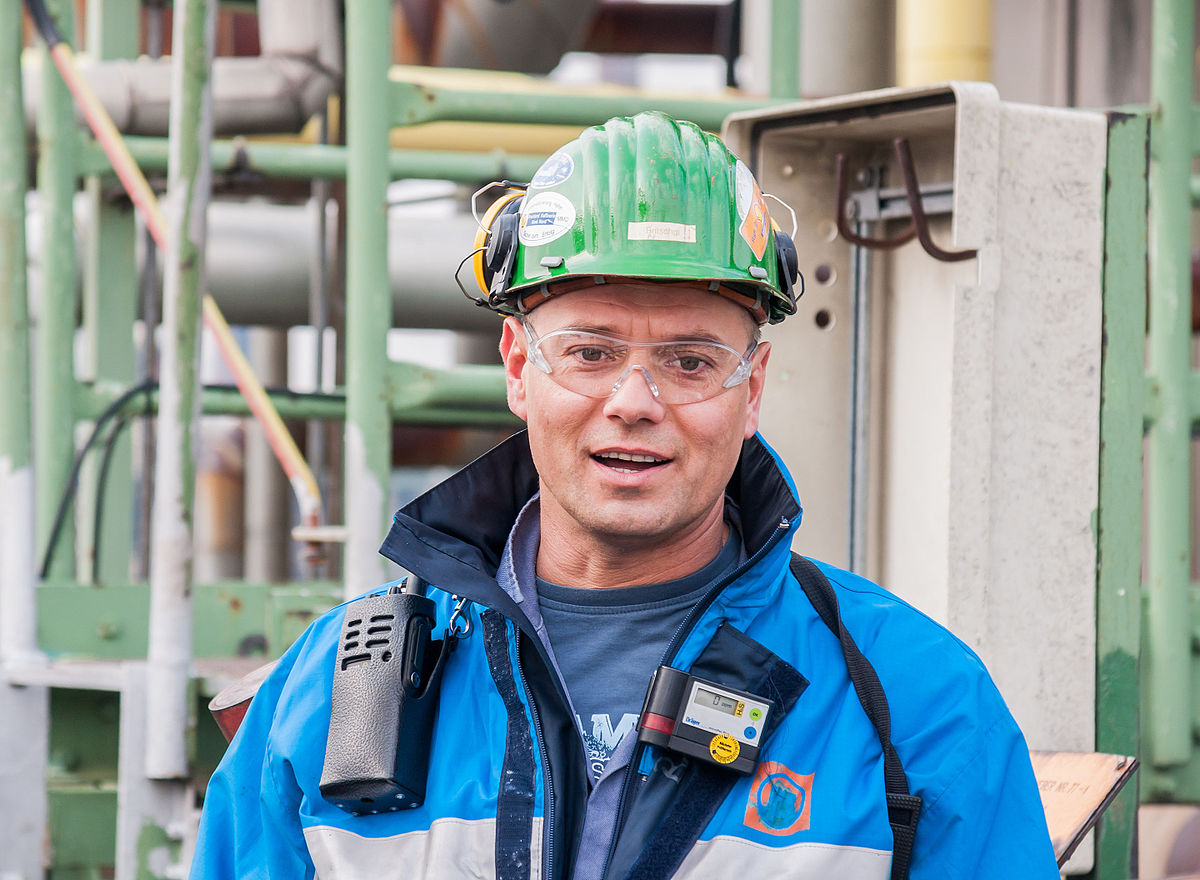
\includegraphics[width=8cm]{hat.jpg}\par
Wearing a hard hat is one of the easiest ways to protect the most important part of your body - the head.
  \end{center}
\subsubsection*{Dielectric Footwear}
Electrical shock resistant (EH) footwear is manufactured with non-conductive electrical shock resistant soles and heals. It must be capable of withstanding the application of 14,000 volts at 60 hertz for one minute with no current flow or leakage current in excess of 3.0 milliamperes, under dry conditions.

According to OSHA, employees must use protective footwear when the employee's feet are exposed to electrical hazards. The employer is responsible for ensuring that each affected employee uses protective footwear when working in areas where there is a danger of foot injuries due to falling or rolling objects, or objects piercing the sole, and where such employee's feet are exposed to electrical hazards.
\begin{center}
  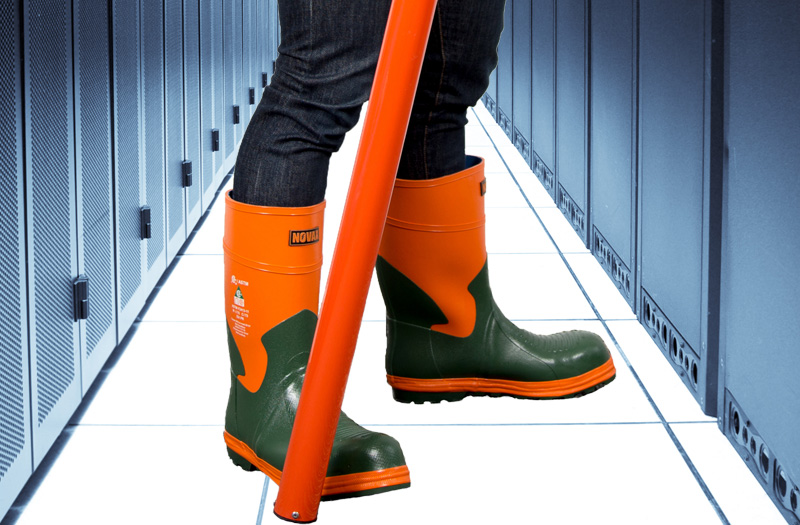
\includegraphics[width=7cm]{boots.jpg}\par
  \end{center}
\subsubsection*{Arc Flash Clothing}
Flame resistant (FR) clothing significantly reduces burn injuries, which can save lives in the event of an accident. If employees are working in a potentially dangerous environment where heat or flame hazards are present, it is the responsibility of the employer to ensure that workers are sufficiently protected. Protective clothing includes items such as shirts, pants, coveralls, hoods, jackets, rainwear, and parkas. Flame resistant clothing is usually made out of cotton, cotton-synthetic blends, synthetics, or leather. Some synthetics are inherently flame resistant while other clothing may be chemically treated for flame resistance. Based upon the test results, arc flash ratings are determined for the clothing based on its resistance to the amount of incident thermal energy to which it is exposed from the arc. The rating assigned is based on the estimated onset of second degree burns.
The arc flash rating is called the Arc Thermal Performance Value (ATPV), which is expressed in calories per square centimeter (cal/cm2) or joules per square centimeter (J/cm2). Clothing is available with ATPV ratings from approximately four to greater than 50 cal/cm2 (16.7 to 209 J/cm2 ).
The arc rating can be found on the clothing label, per the requirements of ASTM F1506. It's important not to confuse protective clothing designed for use against flash fires with clothing that has been designed for use against electric arcs.
\begin{center}
  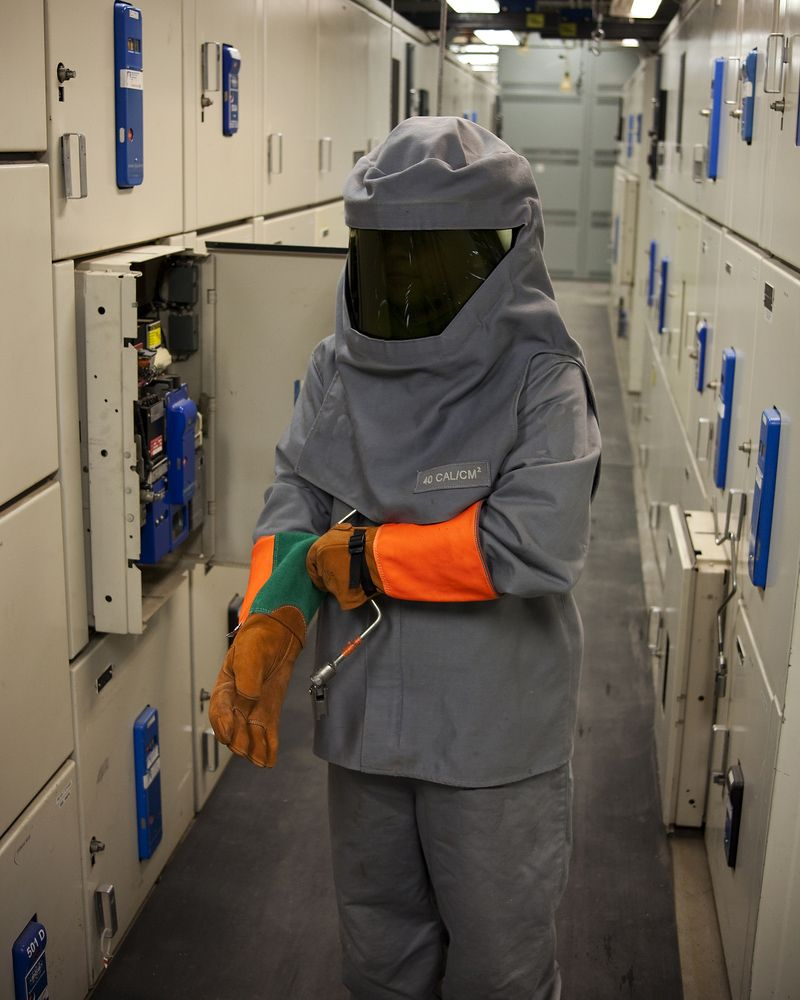
\includegraphics[width=8cm]{arcflashsuit.jpg}\par
  With great power, comes great responsibility.
  \end{center}
\subsubsection*{Rubber Insulating Gloves and Sleeves}
Insulating rubber gloves are among the most important articles of personal protection an electrical worker can wear. To be effective, electrical safety gloves must incorporate dielectric properties and physical strength, along with flexibility and durability.

Rubber is susceptible to the effects of the ozone, which can cause cracking and compromise the integrity of the glove. If the gloves are used in an environment where the levels of ozone are high due to pollution, ozone resistance is critical.

There are two "types" of rubber glove:
\begin{itemize}
    \item Type I glove is not ozone-resistant. These gloves can be negatively affected by ozone and UV rays, rendering them unsafe.
    \item Type II is ozone-resistant. These gloves are not as susceptible to ozone and UV rays, however they are not as flexible as Type I and therefore more uncomfortable to wear.
\end{itemize}

Protective gloves are categorized into six classifications, each based on the approved voltage levels the gloves can provide protection for. Rubber insulating gloves are electrically proof tested at voltage levels specified by ASTM D120-14a prior to being issued.
\begin{center}
  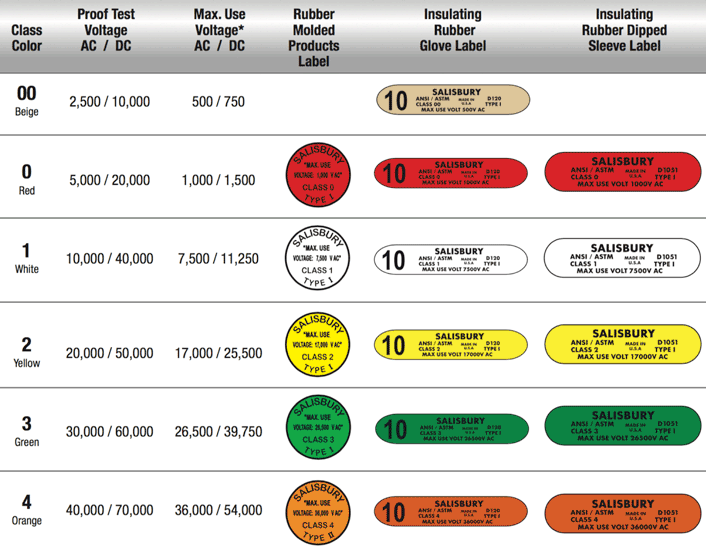
\includegraphics[width=14cm]{gloveschart.png}\par
  \end{center}
\subsection{Isolation \& Lock out / Tag Out}
Modern machinery can contain many hazards to workers from electrical, mechanical, pneumatic or hydraulic energy sources. Disconnecting or making the equipment safe to work on involves the removal of all energy sources and is known as isolation.

"Lock out \& Tag Out" refers to the safety procedure used in industry and research settings to insure that dangerous machines have been properly shut-down and are incapable of being started up again prior to the completion of maintenance or servicing work. It requires that all hazardous energy sources have been:
\begin{enumerate}
    \item identified
    \item isolated
    \item rendered inoperative
\end{enumerate}
to prevent the release of potentially hazardous energy prior to the start of any repair or maintenance procedure. This is accomplished through the locking and tagging of all energy sources. Some common forms of energy isolation include electrical circuit breakers, disconnect switches, ball or gate valves, blind flanges, and blocks. Push buttons, e-stops, selector switches and control panels are not considered proper points for energy isolation.

\begin{center}
  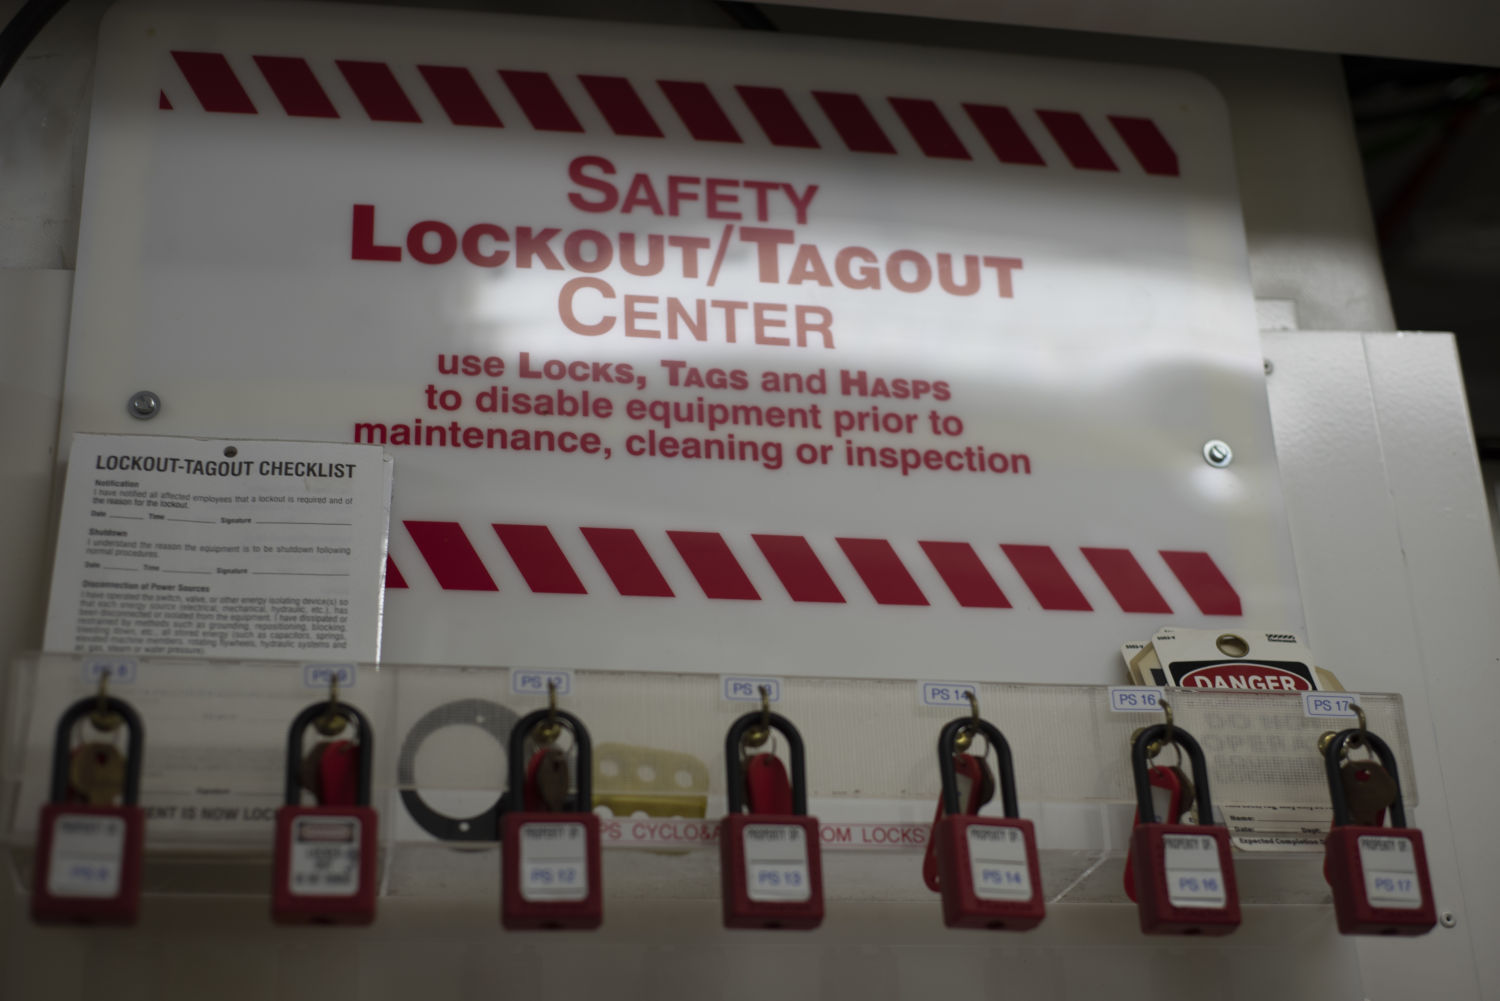
\includegraphics[width=10cm]{newloto.jpg}\par
  A lock out tag out center used on the \textit{MS Noordam}
  \end{center}

Lockout consists of placing a disconnect switch, breaker, valve, spring, pneumatic assemble, or other energy-isolating mechanism in the off or safe position. A device is placed over, around, or through the energy-isolating mechanism to lock it in the off or safe position, and only the person attaching it applies a removable lock to the apparatus.

Tagout is the process by which an energy-isolating device used for lockout is placed in the off or safe position and a written warning is attached to the device or placed in the area immediately adjacent to the device. The tag must identify the person who applied it and be durable and able to withstand the environment in which it is placed. The tag must be substantial so that it can be attached to a variety of locations and will not come off. A tagout device will be used only when the energy-isolating device is not capable of being locked out. The required means of attachment for a tagout device is a self-locking, non-reusable, nylon cable-type tie that is capable of withstanding a 50-lb. force.\cite{ucsb}
Device-specific locks may be used for specific applications where an isolating switch may not be sufficient or, for any reason, is unavailable for use.
\begin{center}Distribution
  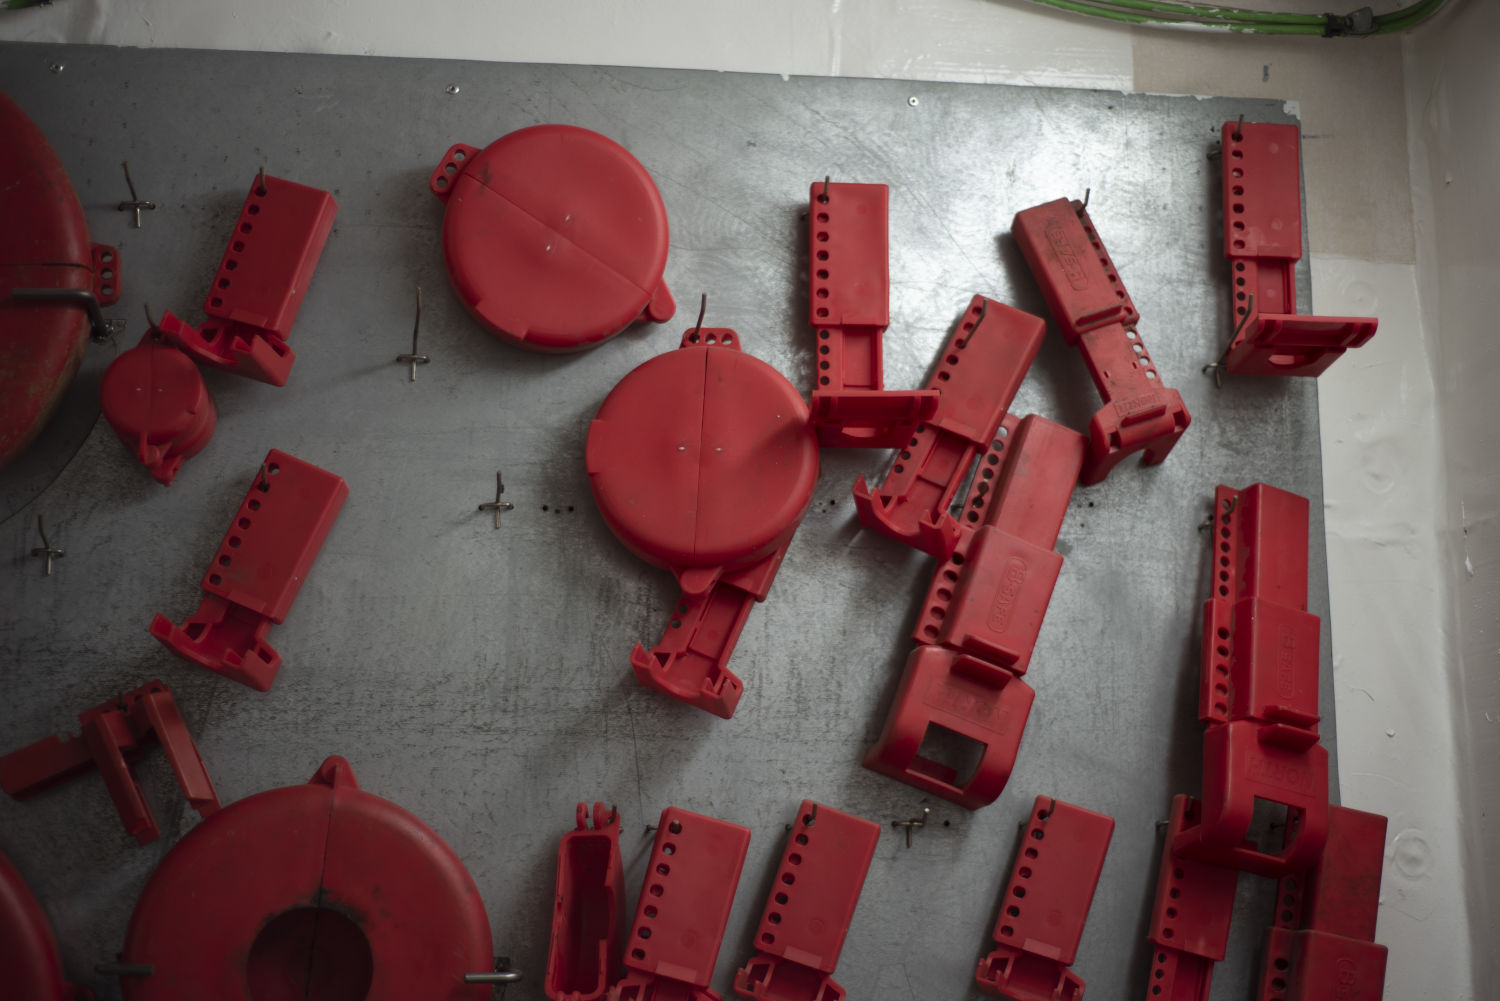
\includegraphics[width=9cm]{lotowall.jpg}\par
  An arrangement of specialized locks used on the \textit{MS Noordam}
  \end{center}

\subsection{Earthing}
Portable earthing devices act a vital part of safety when dealing with high voltage electrical systems. These ensure the protection of personnel  from  dangerous  voltages  that  may  be  caused  by  induced  voltages,atmospheric surges or accidental re-connection of the supply voltage. Isolation  from  supply  voltages  must  be  verified  immediately  before installing portable earthing and short-circuiting devices at the installation point.When  connecting  the  earthing  and  short-circuiting  device, the  earthing cable must be connected to the earthing system first in order to discharge any residual potential or induced voltages.
\begin{center}
  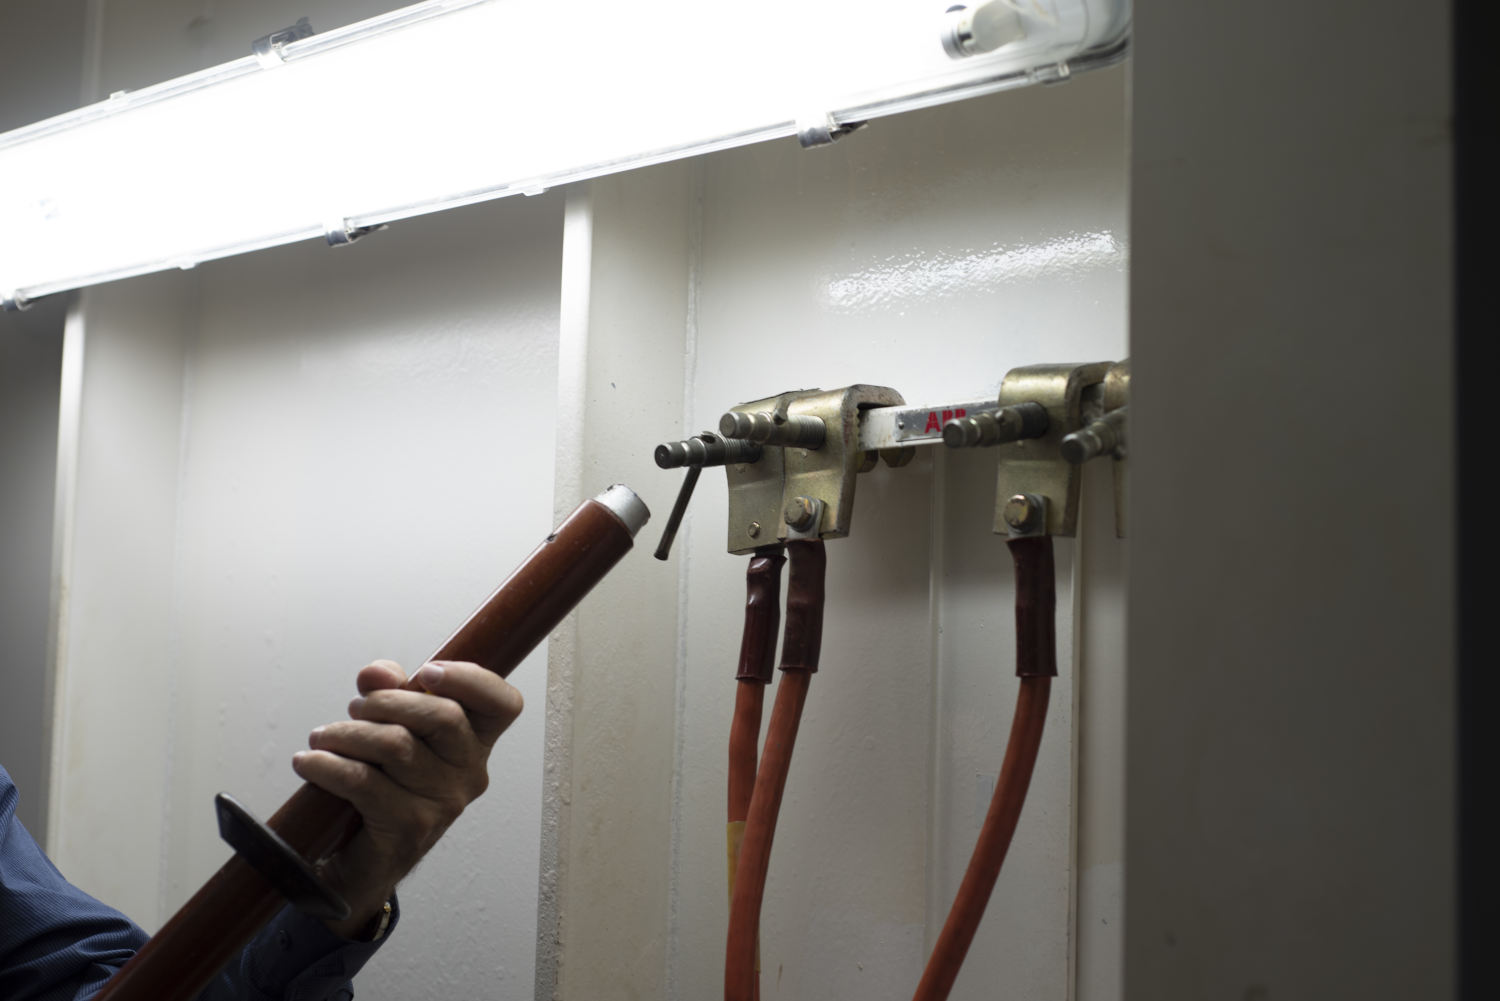
\includegraphics[width=10cm]{noordampeg.jpg}\par
  A portable earthing device used on the \textit{MS Noordam}
  \end{center}
Connection points will be available to mount these tools. Extended insulated rods should be used to safely attach them to the mounting points.
\begin{center}
  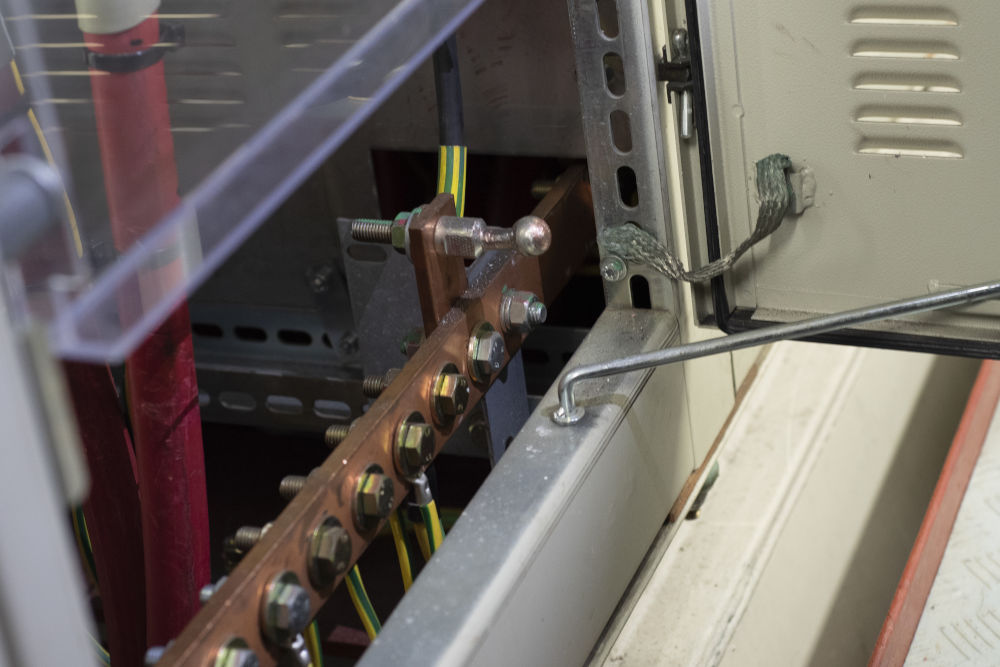
\includegraphics[width=10cm]{peg.jpg}\par
  A earthing mounting peg on the \textit{MS Noordam}
  \end{center}

\subsection{Flammable Areas}
Performing electrical maintenance and repairs in areas where sources of ignition, i.e. electrostatic discharge are considered highly dangerous provides unique challenges for technical staff. According to the IEC, there are four classifications of zones, and consequently have different measures which must be taken to minimize risk. They are:
\begin{itemize}
    \item Class I, zone 0

Locations (1) in which ignitable concentrations of flammable gases or vapors are present continuously or (2) in which ignitable concentrations of flammable gases or vapors are present for long periods of time.
\item Class I, zone 1

Locations (1) in which explosive or ignitable concentrations of flammable gases or vapors are likely to exist under normal operating conditions; (2) in which ignitable concentrations of flammable gases or vapors may exist frequently because of repair or maintenance operations or because of leakages; (3) in which equipment is operated or processes are carried on, of such a nature that equipment breakdown or faulty operations could result in the release of ignitable concentrations of flammable gases or vapors and cause simultaneous failure of electrical equipment in a mode to cause the electrical equipment to become a source of ignition; or (4) that is adjacent to a Class I, Zone 0 location, from which ignitable concentrations of gases or vapors could be communicated, unless such communication is prevented by adequate positive-pressure ventilation from a source of clean air, and effective safeguards against ventilation failure are provided.
\item Class I, zone 2

Locations (1) in which ignitable concentrations of flammable gases or vapors are not likely to occur in normal operation and if they do occur will exist only for a short period; (2) in which volatile, flammable liquids, flammable gases, or flammable vapors are handled, processed, or used, but in which the liquids, gases, or vapors are confined within closed containers or a closed system from which they can escape only in case of accidental rupture or breakdown of such containers or system, or as a result of the abnormal operation of equipment with which the liquids or gases are handled, processed, or used; (3) in which ignitable concentrations of flammable gases or vapors normally are prevented by positive mechanical ventilation, but which may become hazardous because of failure or abnormal operation of the ventilation equipment; or (4) which are adjacent to a Class I, Zone 1 location from which ignitable concentrations of flammable gases or vapors could be communicated unless such communication is prevented by adequate positive-pressure ventilation from a source of clean air, and effective safeguards against ventilation failure are provided.
\item Unclassified

All areas in the facility that are not Zone 0, Zone 1, or Zone 2 are considered unclassified. Arcing electrical equipment in unclassified areas need not be explosion-proof. General-purpose enclosures are acceptable in these areas.
\end{itemize}
There are also unique classifications specifically for explosive dust hazards. These fall under the NEC, are are:
\begin{itemize}
    \item Class II, Division 1 classified locations

    An area where ignitable concentrations of combustible dust can exist all of the time or some of the time under normal operating conditions.

    \item Class II, Division 2 classified locations

    An area where ignitable concentrations of combustible dust are not likely to exist under normal operating conditions.

    \item Class III, Division 1 classified locations

    An area where easily ignitable fibers or materials producing combustible flyings are handled, manufactured or used.

    \item Class III, Division 2 classified locations

    An area where easily ignitable fibers are stored or handled.
\end{itemize}
Following this trend of categories, there are differing levels of safety equipment. The equipment category indicates the level of protection offered by the equipment.
\begin{itemize}
      \item   Category 1 equipment may be used in zone 0, zone 1 or zone 2 areas.

      Very high level of protection; equipment may continue to operate in the presence of explosive atmosphere
      \item       Category 2 equipment may be used in zone 1 or zone 2 areas.

      High level of protection; equipment to be de-energised in presence of explosive atmosphere
        \item     Category 3 equipment may only be used in zone 2 areas.

        Acceptable level of protection; equipment must be removed in presence of explosive atmosphere
    \end{itemize}
\subsection{Interpreting Shipboard Instructions \& Electrical Equipment Safety Guidelines}
Electrical work is dangerous work. To reduce the risk to technical staff, companies will provide documentation, based on the manufacturer's recommendations, on the most effective and safe settings for all configurable systems. These recommendations may be found in the ship's documentation, either on paper in booklets, or computerized in .PDFs. Potentially these may also be online, with shore-side updates being pushed to the ship as soon as they become available, ensuring technical accuracy. These recommendations should only be deviated from with the discretion of the Chief Engineer/Chief Electrician and with approval of the Master, and in some situations, with approval of the manufacturer and/or the shore-based headquarters. Technical staff do not often modify any configuration. Instead, their job is primarily to ensure the effective operation of the existing equipment, as laid out by the manufacturer during the ship's design stage.
\subsubsection*{When in doubt, ask}
Work performed should always be planned in advance. Planning is an essential part of the process, and requires thorough research to be completed successfully. The ship's drawings, diagrams and documentation offer insight to the intended operation of a system, and it will often include specific information relating to a SKU or specifications of any given aspect. For example, a pump may have a series of 2A fuses attached to its control circuit via a transformer. If those fuses require replacing, it is paramount they be replaced with identical ratings. Too high, i.e. 10A, and damage could be done to the circuit. Too low, i.e. 500mA, and the circuit may "nuisance trip" from standard operation. This information may only be available in the ship's drawing, and despite being an extremely simple replacement job, it demands careful consideration.
\newpage
% BEGINNING OF LEARNING OUTCOME 2
\section{Learning Outcome 2}
\begin{tcolorbox}[colback=red!5!white,colframe=red!75!black,title=\textbf{Demonstrate knowledge of and interpret basic electrical drawings.
PERFORMED USING VISIO SOFTWARE AND IN CLASS ANALYSIS. No answers required here. Student to submit Visio drawing file.}]
\begin{itemize}
\item Interprets main features of ships electrical system technical drawings for maintenance and repair purposes.
\item Interprets main features of ships electrical equipment drawings for maintenance and repair purposes.
\item Identifies the symbols for electric generators, motors, transformers, contacts, switches, breakers, relays, time-delay relays, thermal relays, contactors, signal lights, fuses, measurement sensors and electric measuring devices, lighting fixtures, switches, sockets, connection boxes.
\item Identifies the following diagram types: block, system, circuit, wiring (connection), view (layout).
\end{itemize}
\end{tcolorbox}
\textit{Please see submitted materials}
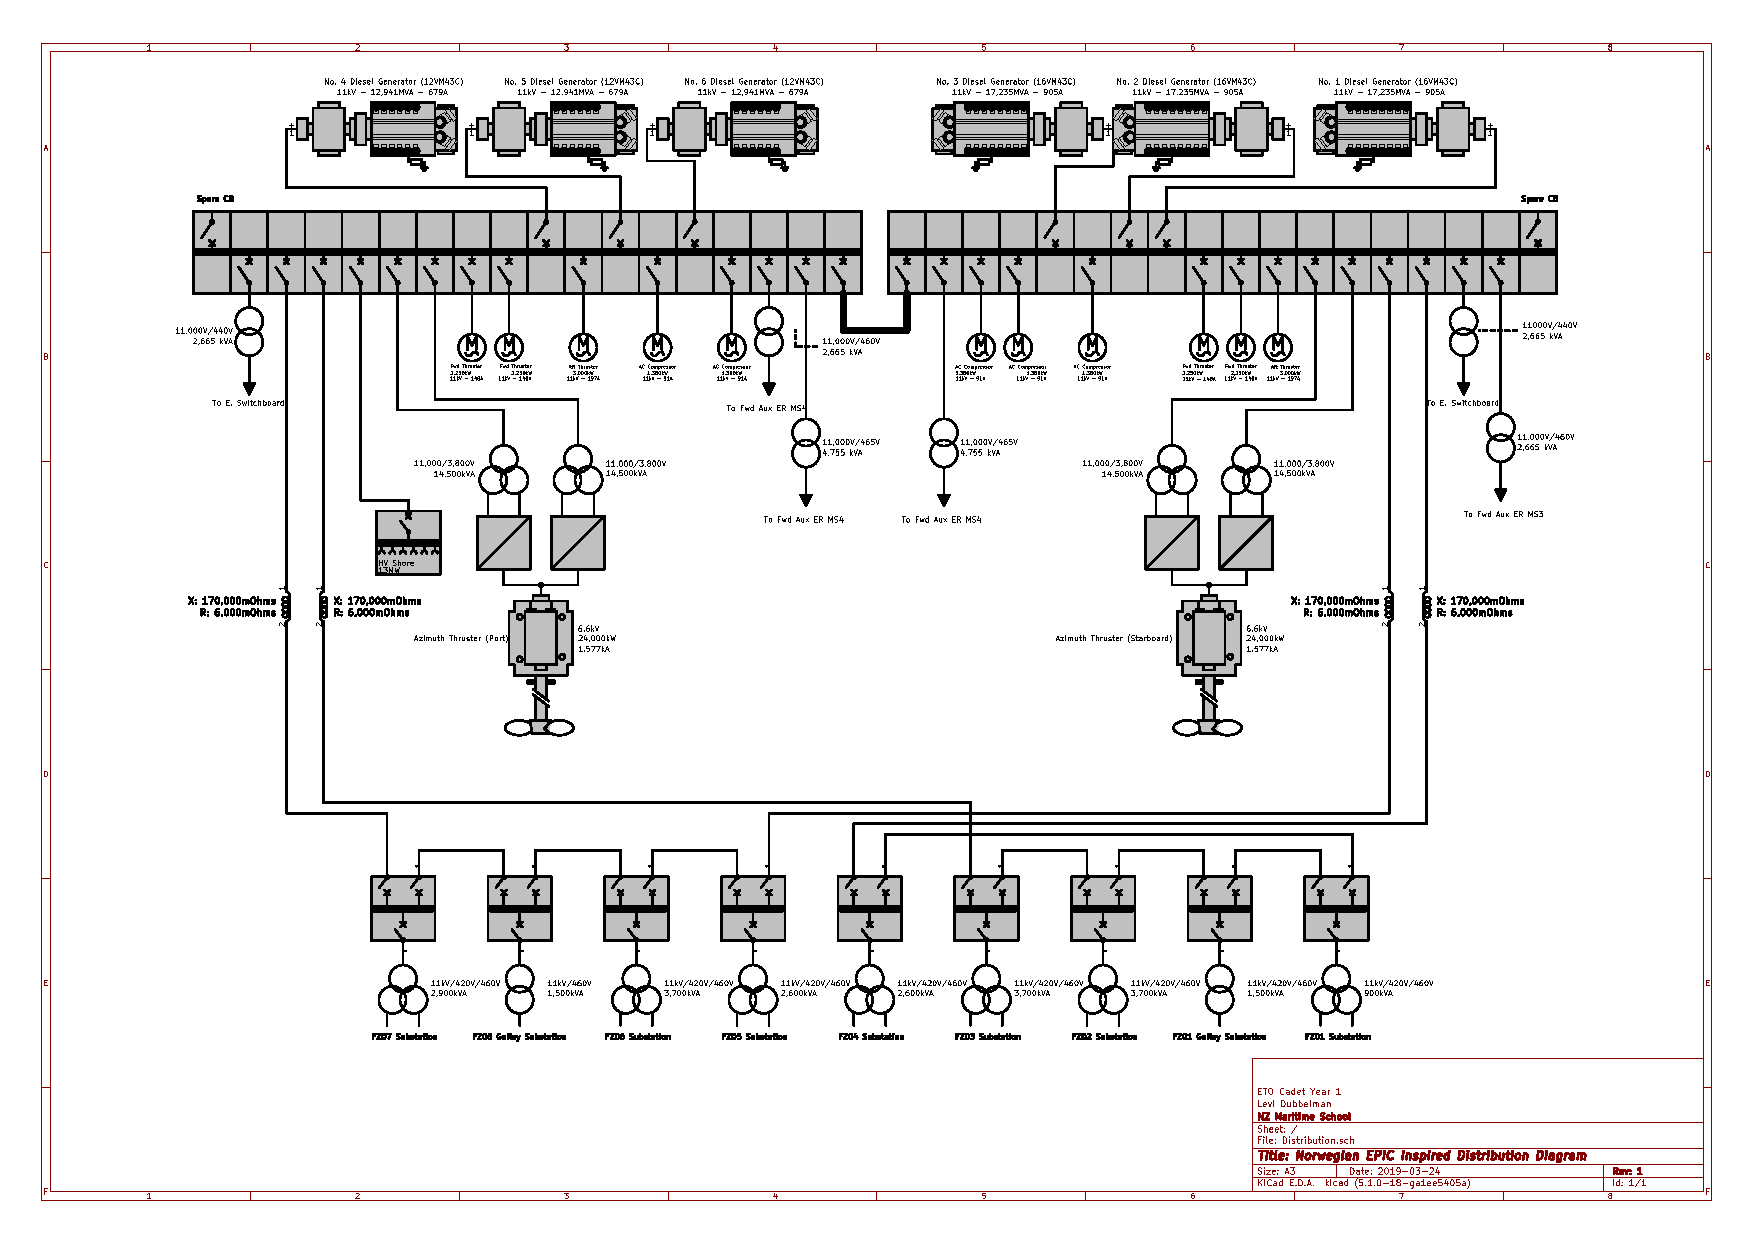
\includepdf[landscape=true]{Distribution.pdf}
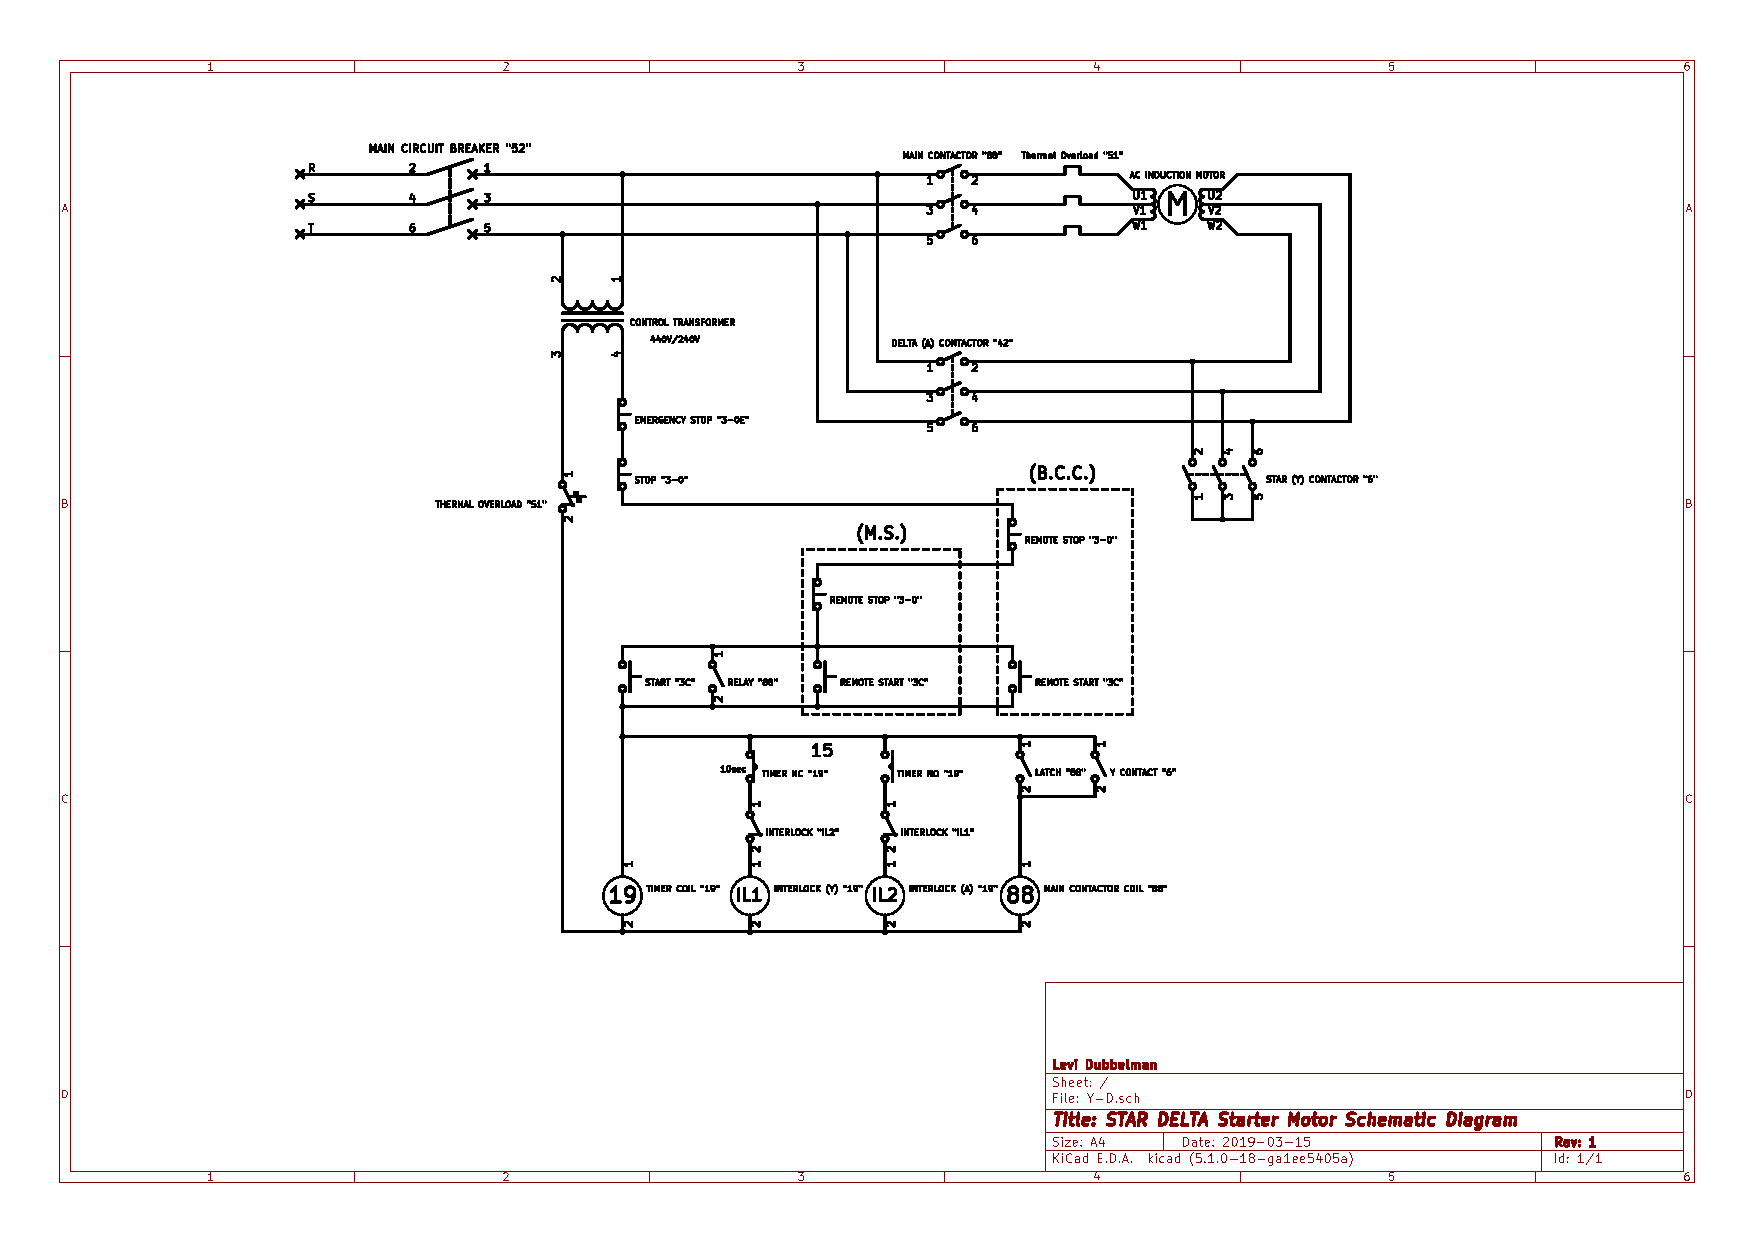
\includepdf[landscape=true]{stardelta.pdf}
\newpage
% BEGINNING OF LEARNING OUTCOME 3
\section{Learning Outcome 3}
\begin{tcolorbox}[colback=red!5!white,colframe=red!75!black,title=\textbf{Test for and detect basic faults and restore electrical equipment and machinery to operating condition}]
\begin{itemize}
\item Explain how to detect basic equipment/machinery electrical malfunction.
\item Explain how to locate basic electrical faults.
\item Explain how to take action to prevent further damage due to a fault.
\item Correctly uses measuring and calibration instruments during testing and restoration. IN LAB.
\item Explain how to interpret and follow shipboard instructions and procedures for fault detection and system/equipment restoration.
\end{itemize}
\end{tcolorbox}
\subsection{Fault Finding}
A simple way to express the principles of fault-finding is with a 5-step system.
\begin{enumerate}
\item Gather Information – Ask as many people as possible who where there,  when \& how the fault occurred
\item Analyse Information – decide the probable cause based on training, and the ship's documentation
\item Investigate – now attempt to find the fault from your analysis
\item Rectify – once found, safely repair the fault
\item Test – when the fault is put right \& restored, test your work before re-energising
\end{enumerate}
\subsubsection{Gather Information}
Constant communication with other members of the crew is critical to gathering the most relevant information possible. It is not guaranteed that you will be able to observe the fault with your own eyes and ears when it occurs, and therefore will need to rely on secondary sources. Occasionally this may be CCTV footage, CANBUS logs or simply by having a discussion with the crew who were present. Asking the right questions-- not badgering the crewmember with irrelevant or pointless details, and not belittling the crewmember by making them feel stupid for not understanding what the fault was, will help you establish a clearer picture of what happened.
\begin{center}
  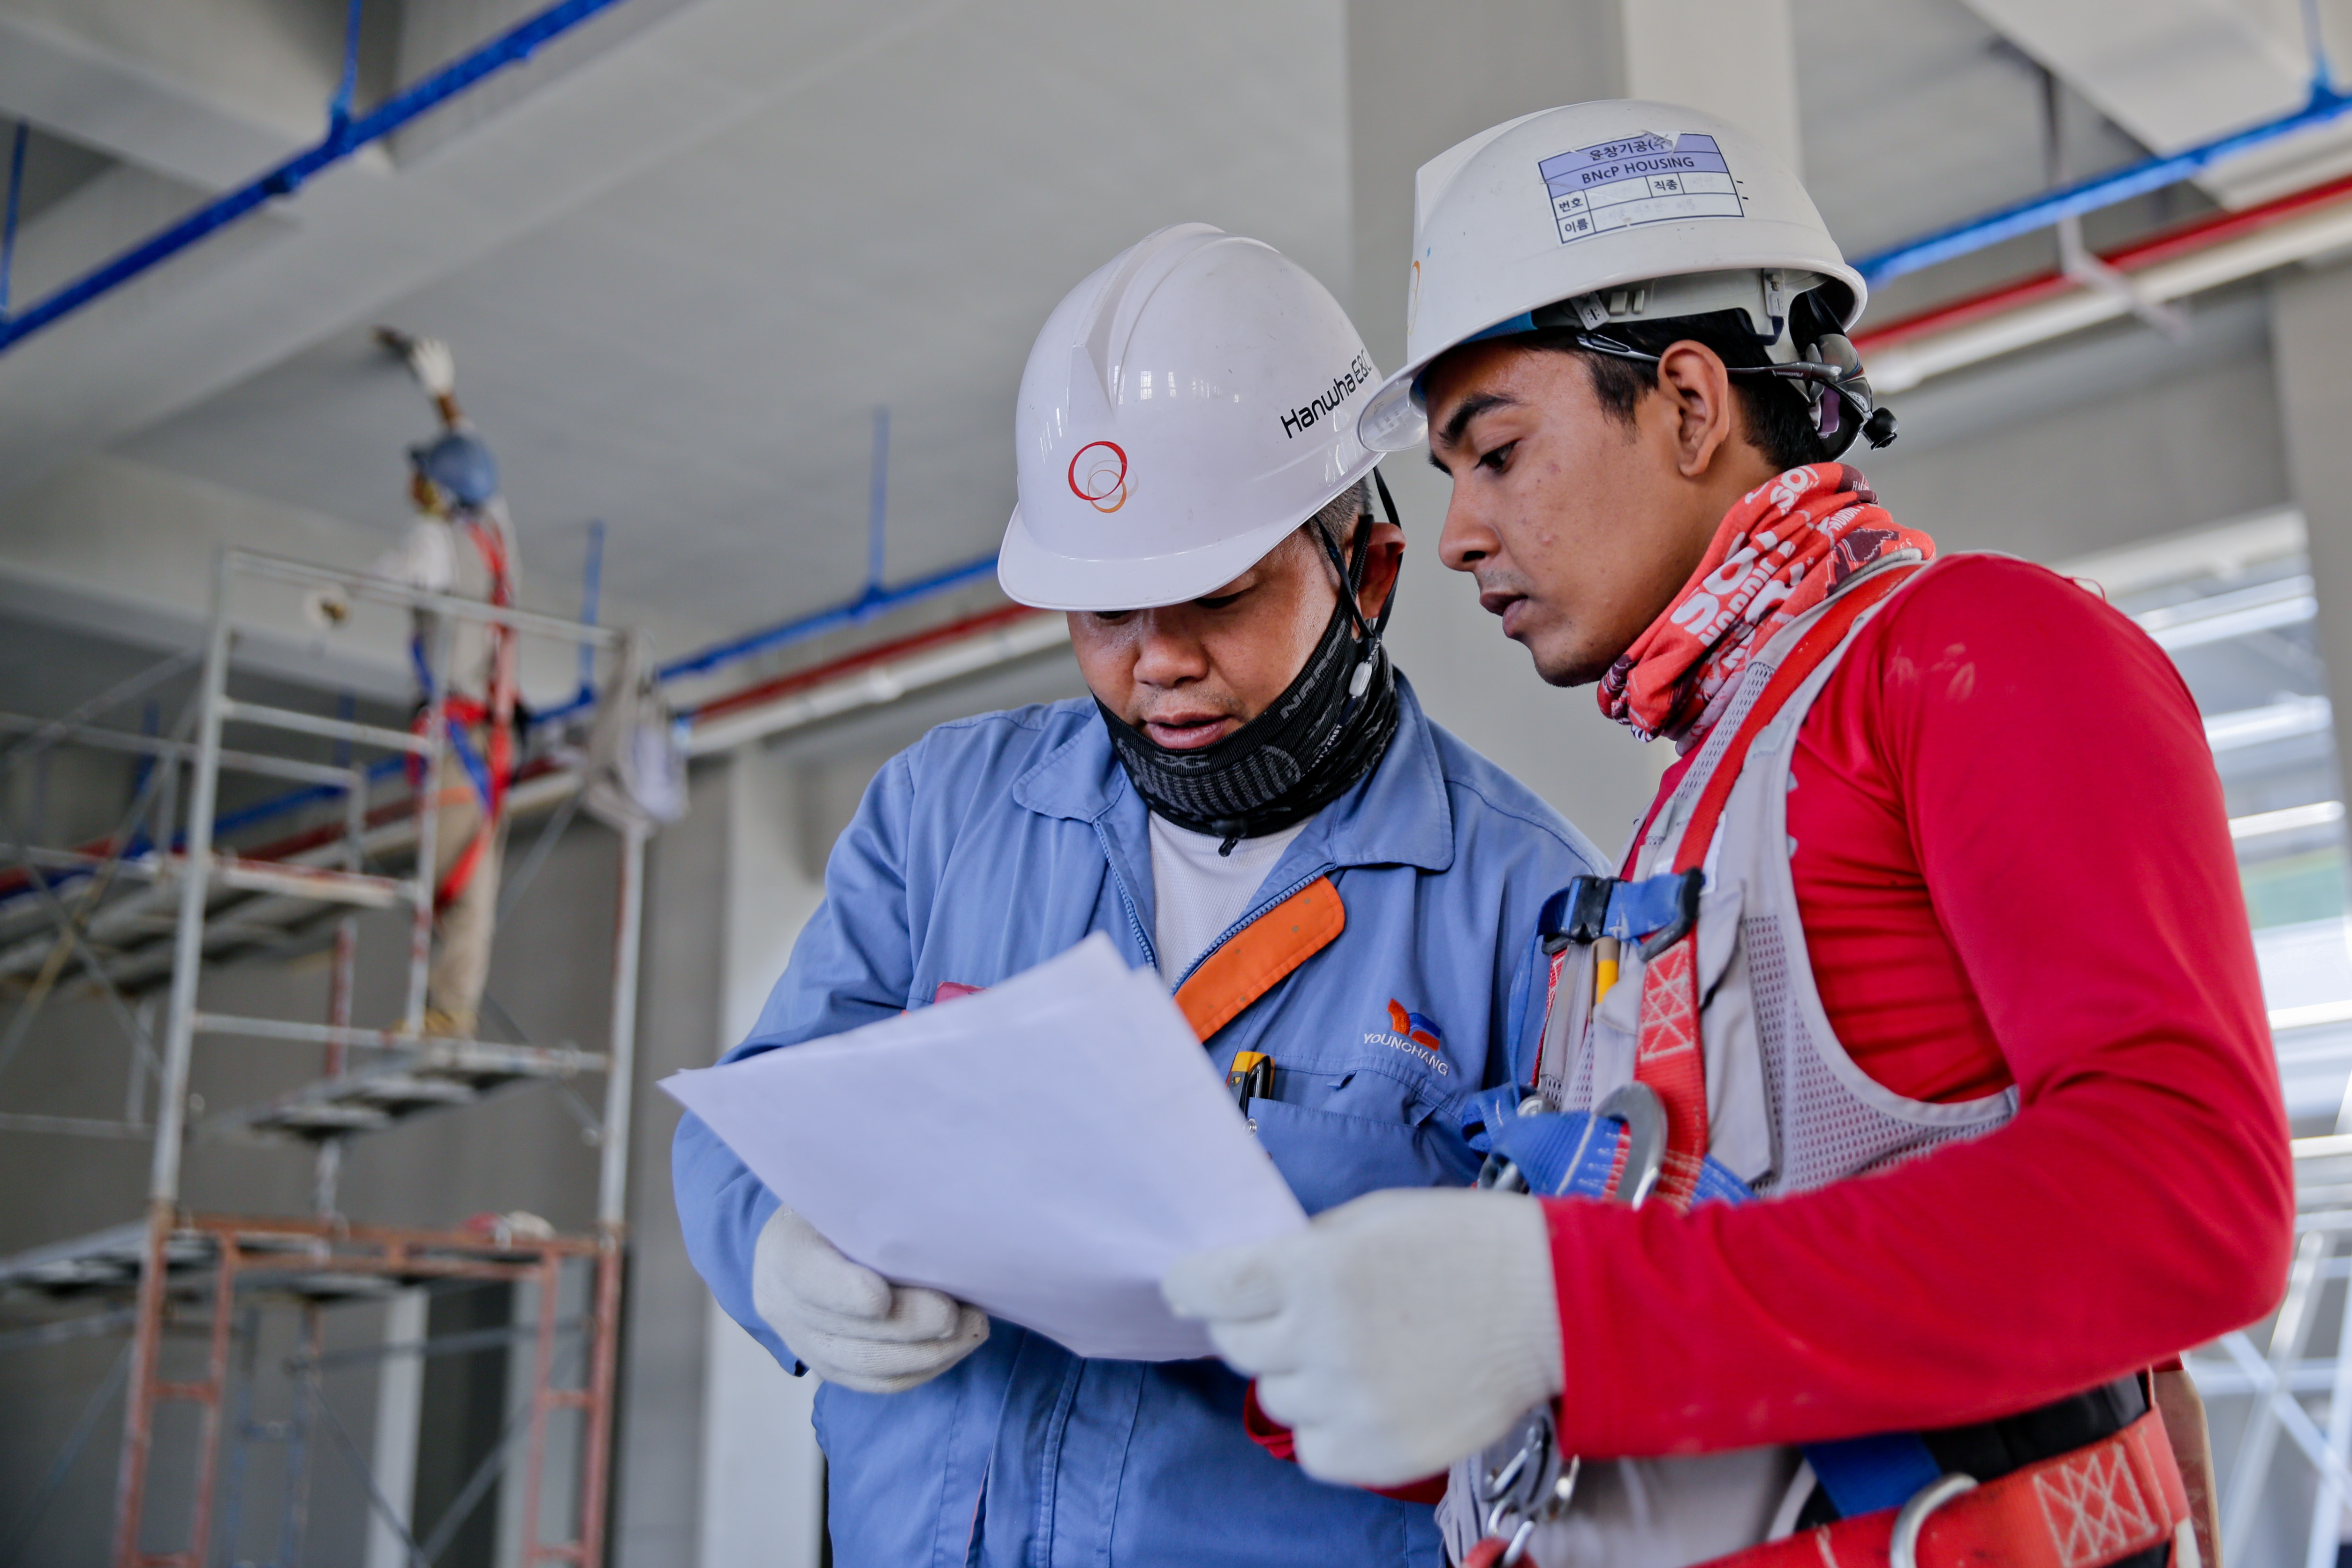
\includegraphics[width=12cm]{menchat}
\end{center}
\subsubsection{Analyse Information}
Taking what you've learned from step 1, try to put together an image of what could have happened based on the evidence. Consult the ship's diagrams and documentation, discuss this with your colleagues (if applicable). This part is critical, as it narrows down the areas where your search takes place, and ensures that your efforts are focussed and effective.
\begin{center}
  
\includegraphics[width=12cm]{manplan}
\end{center}
\subsubsection{Investigate}
\textit{Note: If it hadn't been already, now is a good opportunity to lock out and tag out the faulty system! Ensure your permit-to-works are filed, and you have the approval of your superior.}\par
You've got a general idea of what happened, based on your discussion with others, and have supporting evidence of why you think what you think the problem is. Now you can visit the site where you believe the fault occured, and investigate. Using your measurement tools which have just been tested to be working, such as a multimeter, and being methodically and procedurally testing the circuit, looking for any abnormality, and then ensure you test your tools again, to verify the readings you took. Keep a careful watch for any visible damage, such as burnt insulation, or any smells of burnt insulation.
\begin{center}
  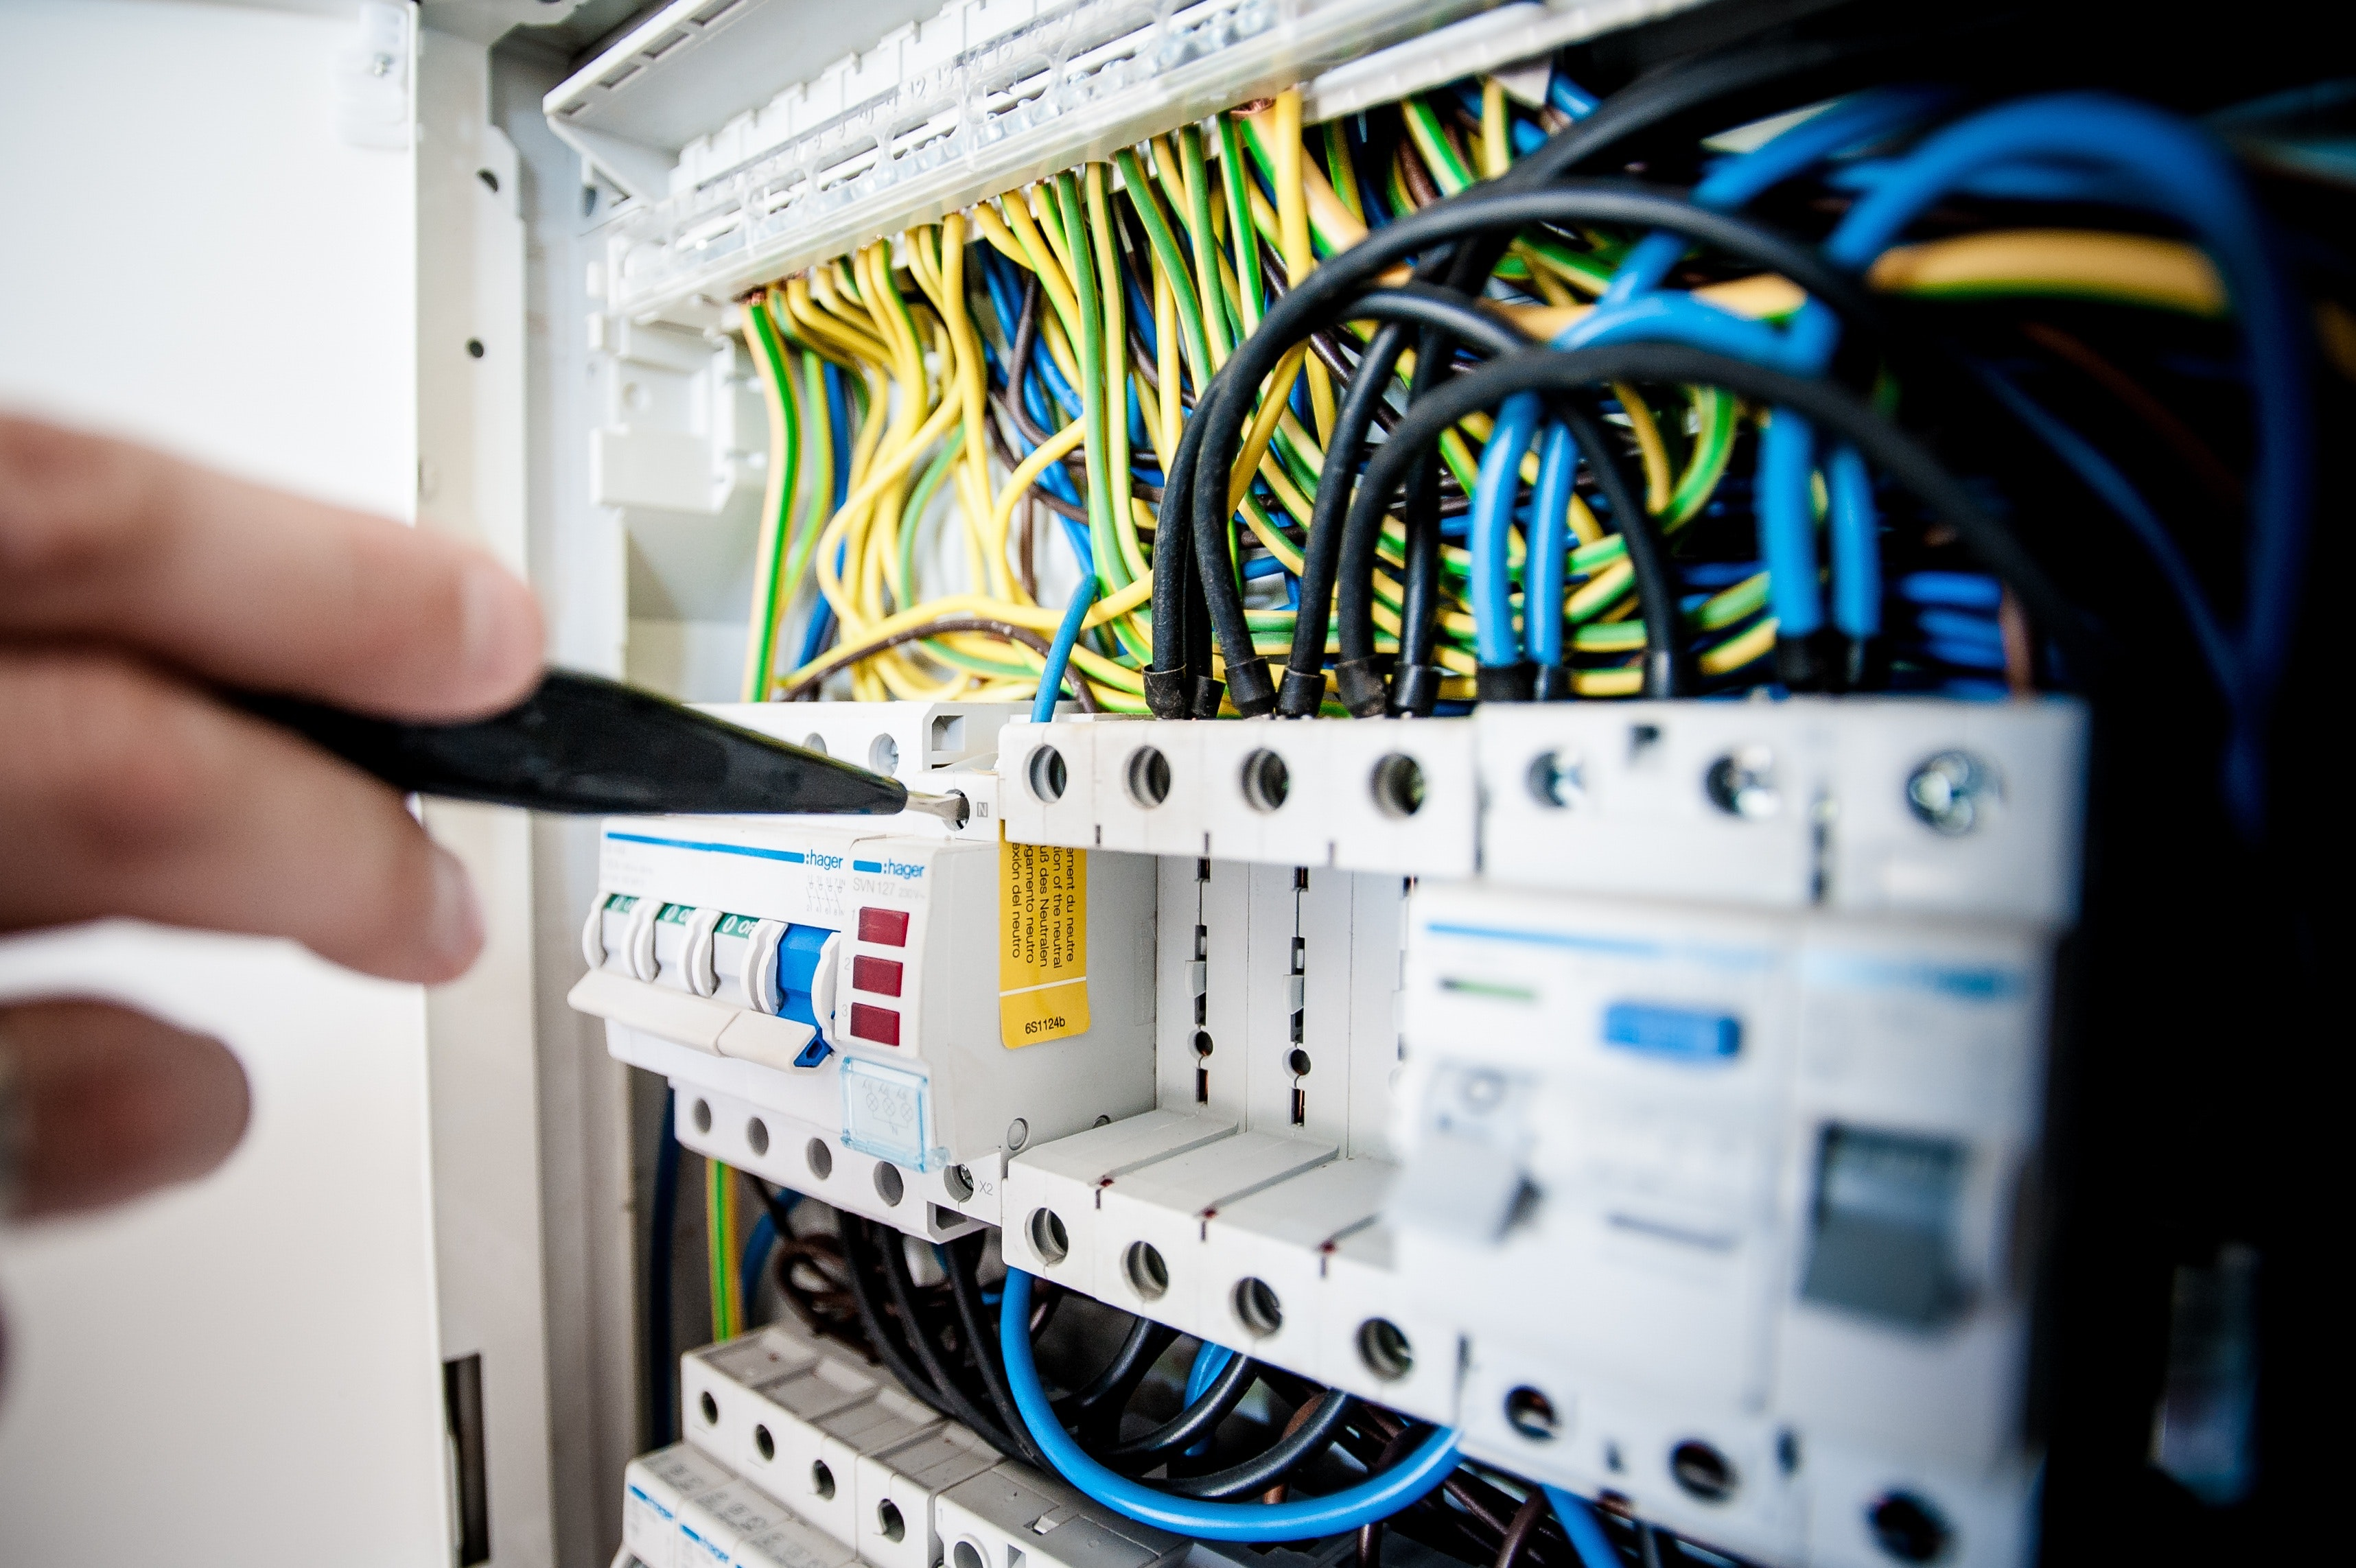
\includegraphics[width=12cm]{multimeter}
\end{center}
\subsubsection{Rectify}
\textit{Note: If you haven't confirmed the fault at this stage, that's okay! Simply repeat the steps as necessary. Gather additional information, analyse it, and continue your investigation!}\par
Now that you've established and confirmed the cause of the fault, it's time to rectify it. In this situation, you may need to replace a faulty component. If you do, ensure that you \textbf{only} replace the component with an \textbf{identical} part. SKUs are a great way to check that parts are the same. If you don't need to replace any components, ensure that your repair work is done carefully, safely and cleanly, you don't want to create additional faults.
\begin{center}
  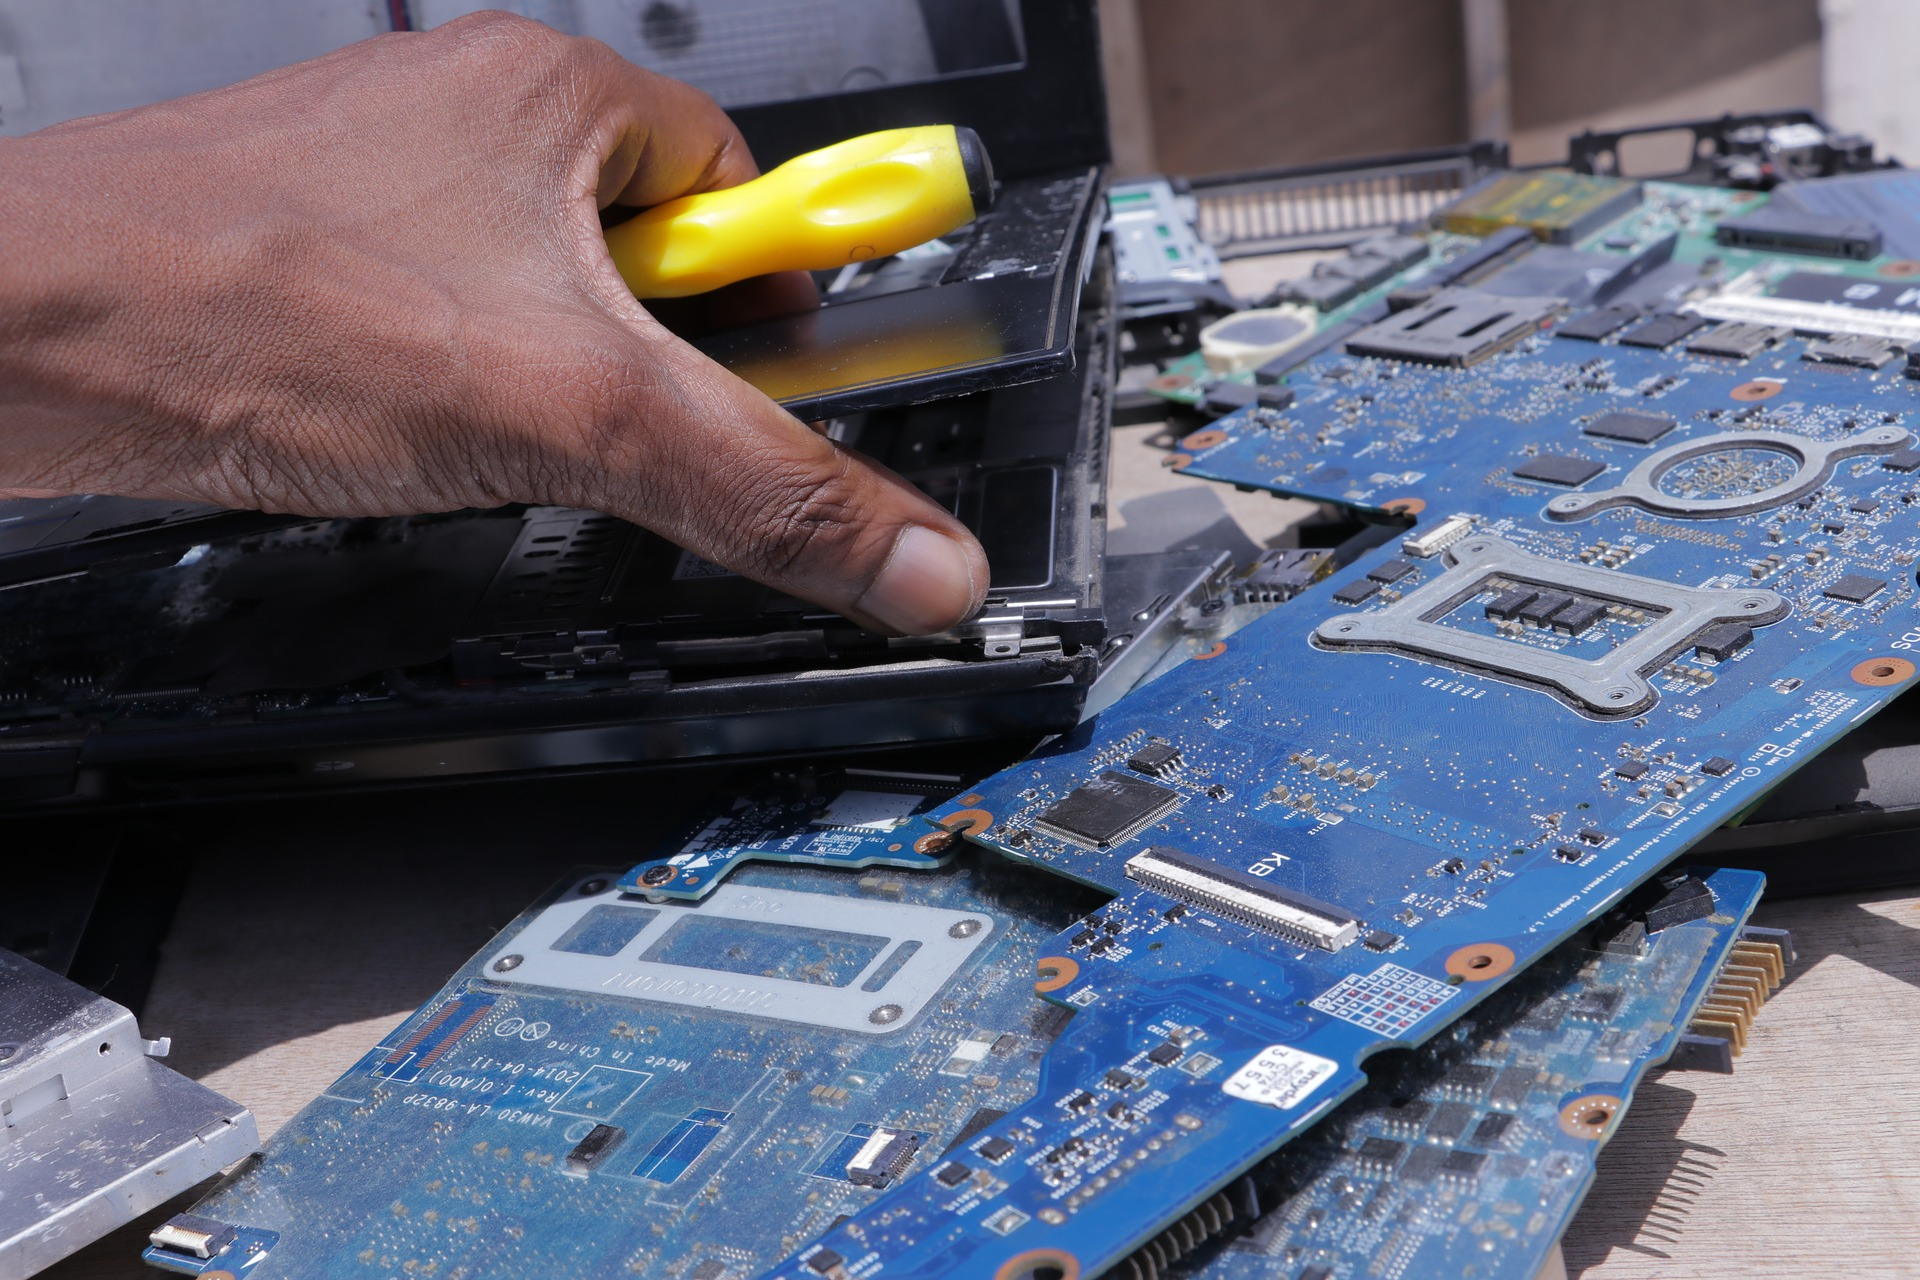
\includegraphics[width=12cm]{fix}
\end{center}
\subsubsection{Test}
If you feel comfortable with your repairs, and they've been checked over by a supervisor, and they're also happy with the quality of work performed, it's time to essentially repeat step 3. Following the same methods you used, ensure the readings you have are correct. File your report, and it's now time to re-energize the (now working) system.
\begin{center}
  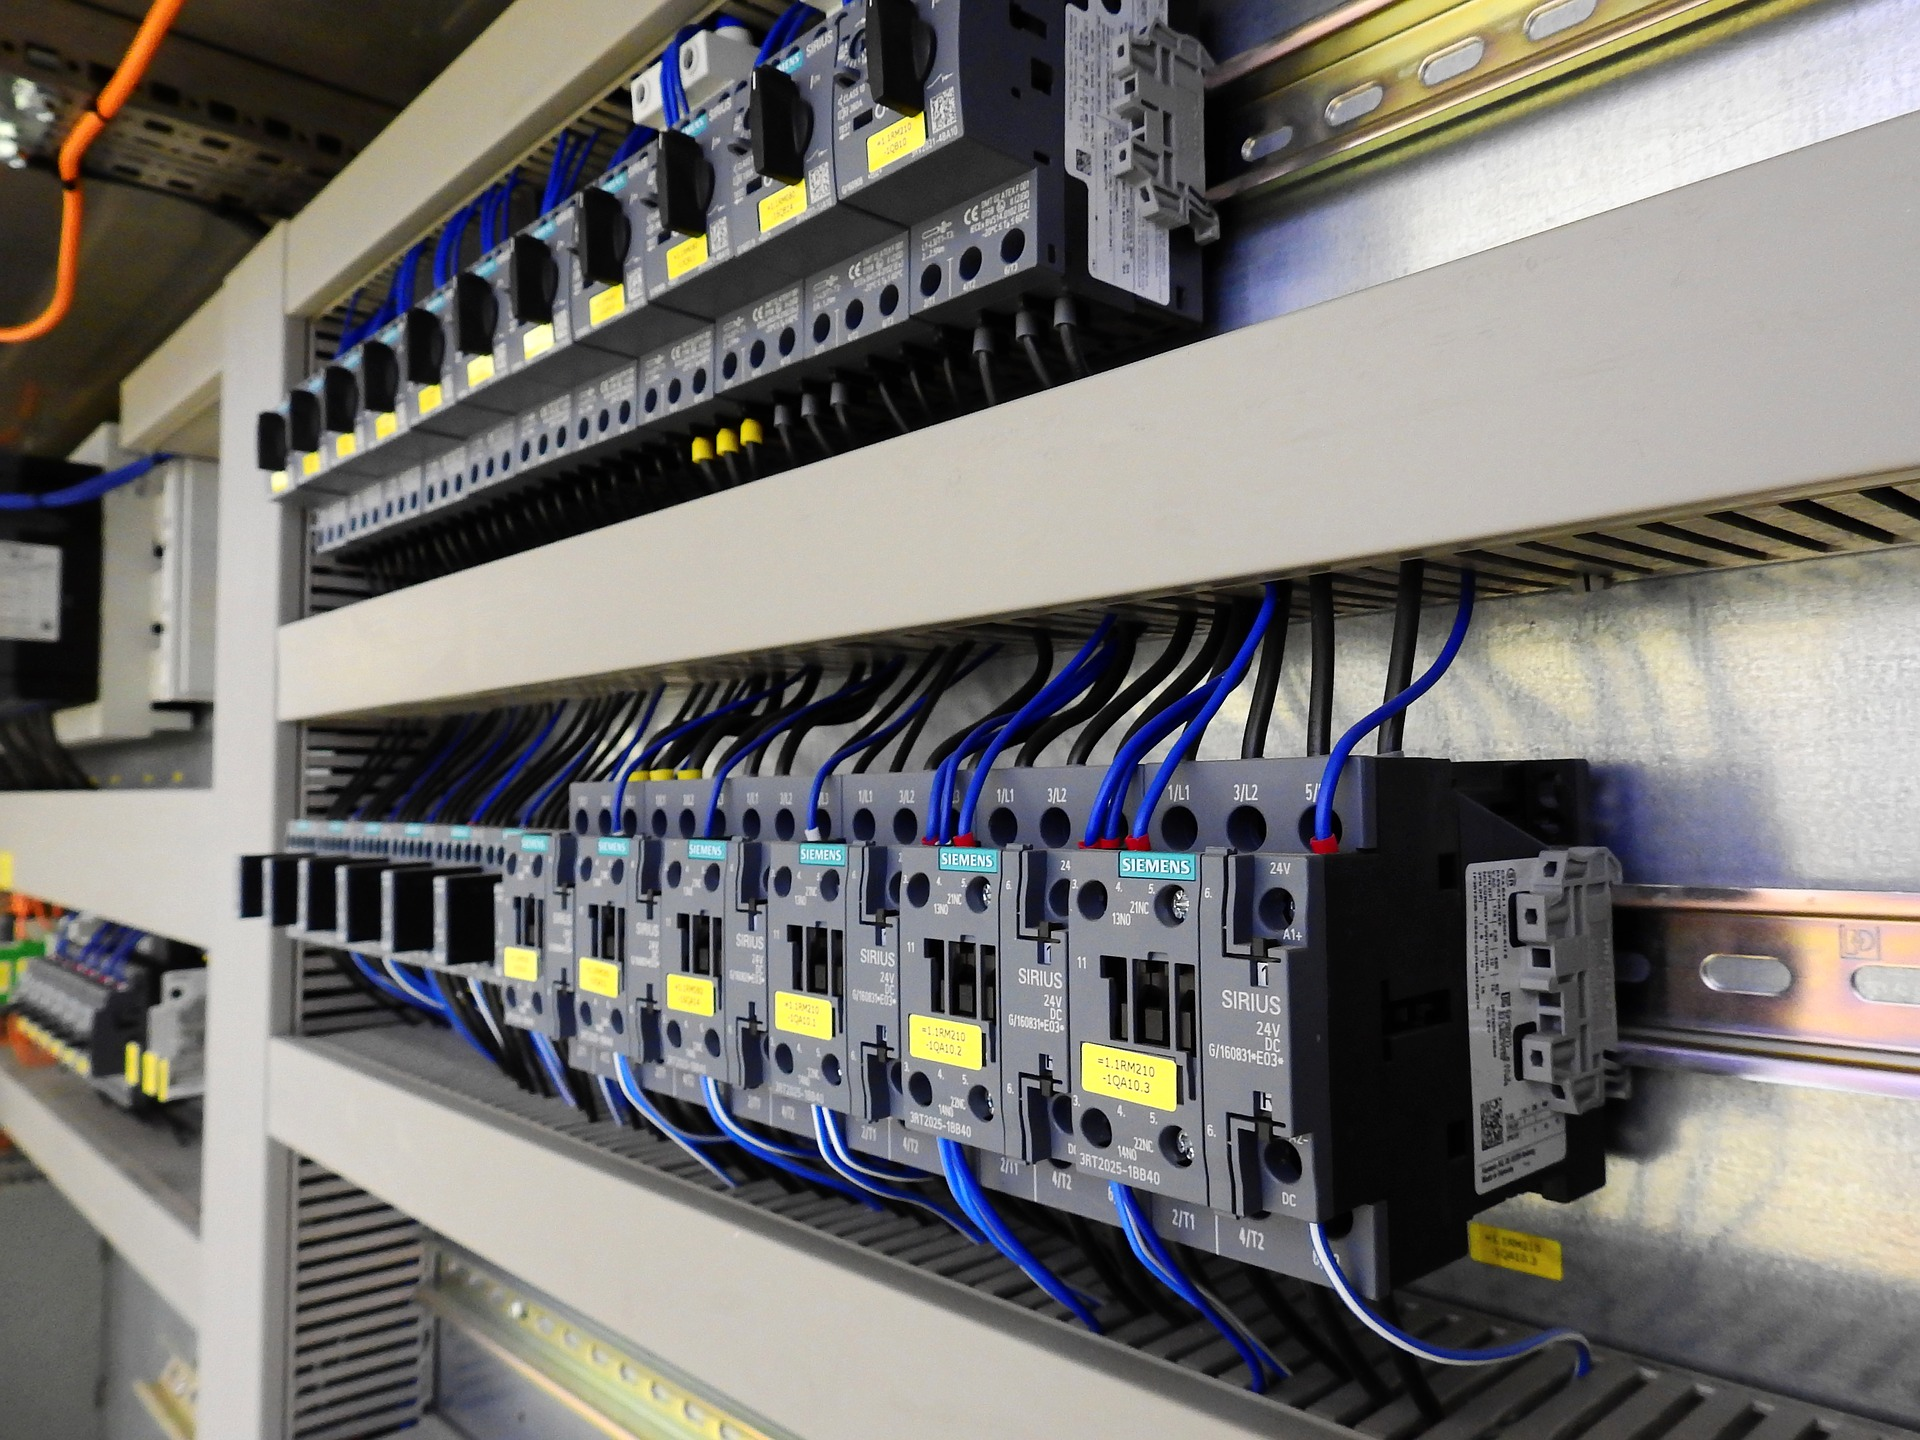
\includegraphics[width=12cm]{energize}
\end{center}
\newpage
% BEGINNING OF LEARNING OUTCOME 4
\section{Learning Outcome 4}
\begin{tcolorbox}[colback=red!5!white,colframe=red!75!black,title=\textbf{Demonstrate knowledge of the basic maintenance requirements of ships fire detection systems}]
\begin{itemize}
\item Interprets typical shipboard electrical fire detection system and maintenance documentation.
\item Knows common fire detection testing procedures.
\item Knows typical fire detection system electrical system preventative maintenance procedures.
\end{itemize}
\end{tcolorbox}
\subsection{Detectors}
Onboard ship, a variety of detection sytems are used, as they all have advantages and disadvantages, depending on the environment where they will be required to operate. Included below is a brief summary of the most effective and common examples of detectors.
\subsubsection{Arc}
\begin{tabular}{|r|l|}
\hline
\textbf{Name} & Arc Flash Detector \\
\textbf{Detection Type} & Pulse of Light (approx. $8,000$ Lux\cite{lux}) \\
\textbf{Detection Time} & $<2ms$ \\
\textbf{Detection Action} & Isolation \\
\textbf{Testing Method} & Built-in testing switch + self testing \\
\textbf{Best Application} & Switchboard Interiors (high voltage) \\
\textbf{Advantages} & Extremely accurate. Extremely fast. Only one unit with multiple I/O. \\
\textbf{Disadvantages} & Cannot detect regular fires. Expensive. Bulky. \\
\hline
\end{tabular}
\begin{center}

\includegraphics[width=6cm]{arcdetector}
\end{center}

\subsubsection{Smoke}
\begin{tabular}{|r|l|}
  \hline
\textbf{Name} & Smoke Detector \\
\textbf{Detection Type} & Optical sensor \\
\textbf{Detection Time} & $>10$ seconds \\
\textbf{Detection Action} & Alarm \& potentially engage fire suppression systems \\
\textbf{Testing Method} & Manual tool which is placed over unit and releases particles \\
\textbf{Best Application} & Areas without steam/smoke, at low risk of fire \\
& e.g. passenger rooms, accomodation\\
\textbf{Advantages} & Inexpensive. Low maintenance requirement. \\
\textbf{Disadvantages} & Susceptible to nuisance tripping. Slow. \\
  \hline
\end{tabular}
\begin{center}
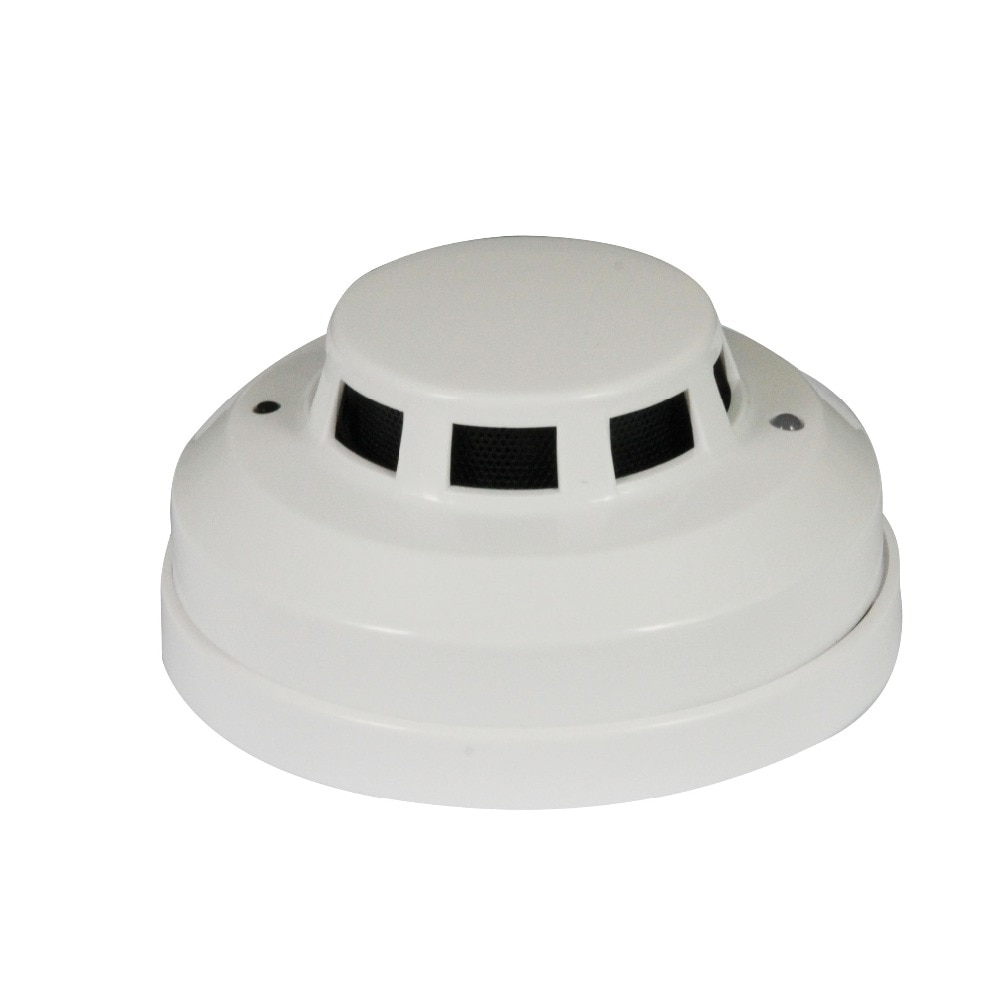
\includegraphics[width=4cm]{smokedetector}
\end{center}

\subsubsection{Flame}
\begin{tabular}{|r|l|}
  \hline
\textbf{Name} & Flame Detector \\
\textbf{Detection Type} & Wavelength of fire \\
\textbf{Detection Time} & $2-3$ seconds \\
\textbf{Detection Action} & Alarm \& fire suppression systems \\
\textbf{Testing Method} & Manual testing lamp \\
\textbf{Best Application} & Machinery/chemical pipes \\
\textbf{Advantages} & Generally accurate. Relatively fast. \\
\textbf{Disadvantages} & Susceptible to nuisance tripping from sunlight. Expensive. \\
\hline
\end{tabular}
\begin{center}
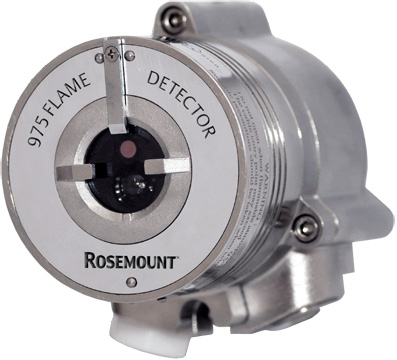
\includegraphics[width=6cm]{flamedetector}
\end{center}
\subsubsection{Heat}
\begin{tabular}{|r|l|}
\hline
\textbf{Name} & Thermal Detector \\
\textbf{Detection Type} & Temperature (Typically $>50$ degrees celsius at device \\
& rate at which temperature increases is factored in) \\
\textbf{Detection Time} & $>15$ seconds \\
\textbf{Detection Action} & Fire alarm \& potentially engage fire suppression systems \\
\textbf{Testing Method} & Manual testing tool placed over unit and produces heat \\
\textbf{Best Application} & In combination with other detectors \\
\textbf{Advantages} & Provides additional level of detection. Cheap. \\
\textbf{Disadvantages} & Very slow. Not effective by themselves.\\
\hline
\end{tabular}
\begin{center}
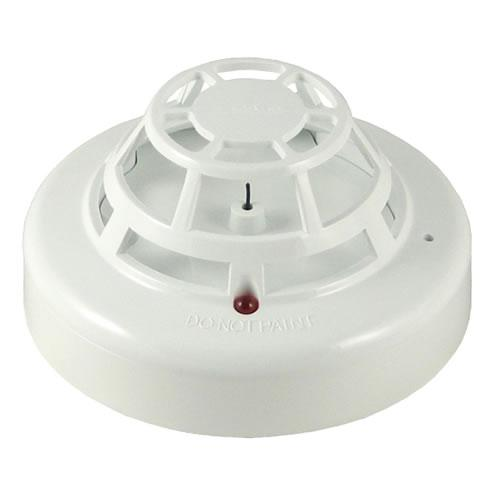
\includegraphics[width=6cm]{heatdetector}
\end{center}
\newpage
\subsection{Fire Suppression Systems}
\subsubsection{Water Mist / Hi-Fog\textregistered}
\begin{tabular}{|r|l|}
\hline
\textbf{Name} & Water Mist / Hi-Fog\textregistered \\
\textbf{Method of Attack} & Oxygen displacement + heat dissipation\\
\textbf{Suppression Type} & Water particles (Hi-Fog\textregistered: approx. 140 BAR)  \\
\textbf{Suppression Time} & $<1$ Minute  \\
\textbf{Testing Method} & Self-testing + regular maintenance discharge \\
\textbf{Best Application} & Directly above high risk systems (e.g. main generators)\\
\textbf{Advantages} & Non-conductive. Extremely fast. \\
& Safe (staff may be present while discharging).  \\
& 400x better than standard sprinklers.\\
\textbf{Disadvantages} & Expensive. Pump array is quite large. \\
& Doesn't scale ship-wide very well.\\
\hline
\end{tabular}
\begin{center}
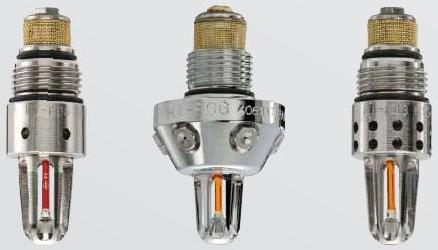
\includegraphics[width=8cm]{hifog}
\end{center}
\subsubsection{Sprinkler}
\begin{tabular}{|r|l|}
\hline
\textbf{Name} & Sprinklers\\
\textbf{Method of Attack} & Heat dissipation\\
\textbf{Suppression Type} & Water particles (approx. $2-3.5$ BAR)  \\
\textbf{Suppression Time} & \textit{Potentially indefinite.}\\
\textbf{Testing Method} & Regular maintenance discharge\\
\textbf{Best Application} & Non-critical areas, when used in conjunction with $CO_2$\\
\textbf{Advantages} & Inexpensive. Reasonably effective against small fires. \\
\textbf{Disadvantages} & Not ideal for larger, or electrical fires.\\
\hline
\end{tabular}
\begin{center}
\includegraphics[width=6cm]{sprinkler.jpg}
\end{center}
\subsubsection{$CO_2$}
\begin{tabular}{|r|l|}
\hline
\textbf{Name} & $CO_2$\\
\textbf{Method of Attack} & Oxygen displacement\\
\textbf{Suppression Type} & $CO_2$ Gas\\
\textbf{Suppression Time} & $10-15$ seconds + time for headcount\\
\textbf{Testing Method} & Regular maintenance on valves. Discharge canisters. \\
\textbf{Best Application} & As a last resort, everywhere.\\
\textbf{Advantages} & Relatively quick. Completely displaces oxygen, smothering fire.\\
\textbf{Disadvantages} & No cooling effect (danger of re-ignition). \\
& Asphyxiating (deadly). Potential source of ESD.\\
\hline
\end{tabular}
\begin{center}
\includegraphics[width=8cm]{co2}
\end{center}
\subsubsection{Extinguishers}
\begin{tabular}{|r|l|}
\hline
\textbf{Name} & Handheld/portable Fire Extinguishers \\
\textbf{Method of Attack} & Various types. Usually oxygen displacement.\\
\textbf{Suppression Type} & Various types. Usually either $CO_2$, or dry/wet chemical \\
\textbf{Suppression Time} & Instant, if applied to base of fire.\\
\textbf{Testing Method} & Pressure indicator gauge\\
\textbf{Best Application} & Allowing staff to escape fire, last-ditch attempts at suppression\\
\textbf{Advantages} & Inexpensive. Portable. Generally effective for small fires.\\
\textbf{Disadvantages} & Not ideal for larger fires. Places person at great risk.\\
\hline
\end{tabular}
\begin{center}
\includegraphics[width=12cm]{extin}
\end{center}
\newpage
\begin{thebibliography}{9}
\bibitem{hallswitchboards}
Hall, Dennis T.
\textit{Practical Marine Electrical Knowledge,} $3^{rd}$ ed., Witherby Publishing Group Ltd, 2014.

\bibitem{cutnell}
Cutnell, John D., Johnson, Kenneth W. Physics. 4th ed. New York, NY: Wiley, 1998.
\bibitem{carr}
Carr, Joseph J. Safety for electronic hobbyists. Popular Electronics. October 1997. as found in Britannica.com.

\bibitem{lux}
Schneider Electric, What is the minimum Lux required for arc flash detection using a point sensor for a VAMP 321, 221, or 50 series relay?
https://www.schneider-electric.com/en/faqs/FA180091/

\bibitem{ucsb}
The Regents of the University of California, Energy Isolation / Lock-Out / Tag-Out Program 2018
https://www.ehs.ucsb.edu/general-safety/energy-isolation-lock-out-tag-out
\end{thebibliography}
\end{document}
